% Author: Alejandro Santomé Valverde

\chapter{Fundamentals of Programmable Integrated Photonics} \label{chap:fundamentals}

\section{Fundamentals of Integrated Photonics} \label{sec:fundamentals-int_photonics}

Integrated photonics aims to generate, guide, manipulate, and detect optical signals within a 
compact and scalable platform by integrating multiple photonic components on a single substrate. 
By leveraging waveguiding structures with high refractive index contrast, photonic integrated 
circuits enable strong optical confinement and precise control of light propagation over 
centimeter-scale distances within chip-scale footprints. This approach provides a robust and 
reproducible alternative to bulk and fiber-based optical systems, while benefiting from wafer-scale 
fabrication and compatibility with semiconductor manufacturing processes 
\cite{sorefPresentFutureSilicon2006,thomsonRoadmapSiliconPhotonics2016}.

The fundamental building block of integrated photonics is the optical waveguide, which confines 
light through total internal reflection enabled by the refractive index contrast between a 
high-index core and a lower-index cladding. Depending on geometry and wavelength, waveguides may 
support single-mode or multi-mode propagation. The propagation of light along a guided mode is 
described by its propagation constant $\beta$, related to the effective refractive index 
$n_{\mathrm{eff}}$ as:

\begin{equation}
\beta = k_0 n_{\mathrm{eff}},
\end{equation}

where $k_0 = 2\pi / \lambda$ is the free-space wavenumber and $\lambda$ is the optical wavelength. 
The accumulated optical phase over a waveguide section of length $L$ is therefore given by:

\begin{equation}
\phi = \beta L = \frac{2\pi}{\lambda} n_{\mathrm{eff}} L.
\end{equation}

Controlled phase accumulation constitutes the physical basis of interferometric and resonant 
devices, which are widely used in integrated photonic circuits.

The main physical building blocks encountered in integrated photonics are summarized in 
Fig.~\ref{fig:ch2-photonics_summary}. These include waveguide confinement and guided modes, 
representative passive components for power distribution and routing, and interferometric or 
resonant structures enabling phase-sensitive functionality.

\begin{figure}[t]
    \centering
    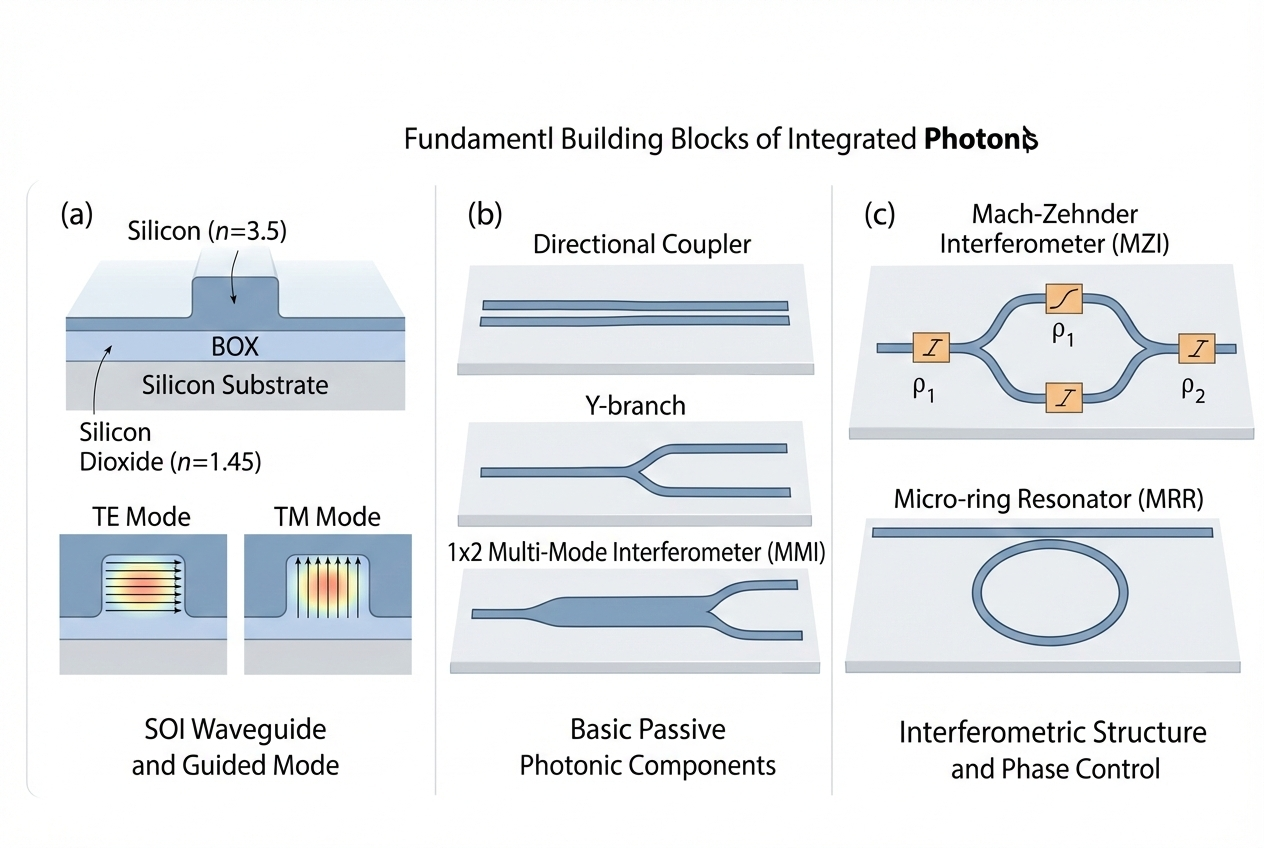
\includegraphics[width=\linewidth]{figures/ch2-photonics_summary.png}
    \caption{Fundamental building blocks of integrated photonics. 
    (a) Cross-section of a generic silicon-on-insulator waveguide and representation of the 
    fundamental TE and TM guided modes. 
    (b) Examples of passive photonic components including a directional coupler, a Y-branch, and 
    a 1x2 multi-mode interferometer. 
    (c) Mach-Zehnder interferometer and a micro-ring resonator.}
    \label{fig:ch2-photonics_summary}
\end{figure}

Different material platforms have been developed to implement integrated photonic circuits, 
including silicon, silicon nitride, and III-V semiconductor technologies. The choice of platform 
determines key parameters such as refractive index contrast, propagation loss, dispersion, thermal 
response, and compatibility with active functionalities. These technological aspects directly 
influence the achievable integration density, power consumption, and scalability of photonic 
circuits \cite{blumenthalSiliconNitrideSilicon2018,bogaertsSiliconPhotonicsCircuit2018}.

From a functional perspective, integrated photonic circuits are composed of passive elements that 
define optical paths and spectral responses, and active elements that enable dynamic control of 
optical signals. Phase shifters, modulators, and photodetectors allow external electrical signals 
to modify or monitor the optical state of the circuit. As the number of components increases, the 
interplay between optical confinement, phase control, losses, and fabrication variability becomes 
increasingly critical.

Loss mechanisms play a central role in determining the scalability of integrated photonic circuits. 
Propagation losses due to material absorption, sidewall roughness, and scattering, together with 
excess losses introduced by bends, couplers, and crossings, accumulate as circuit depth increases
\cite{suScalabilityLargeScalePhotonic2023}. In large-scale circuits, loss accumulation limits 
usable complexity and directly impacts signal-to-noise ratio and energy efficiency.

In summary, integrated photonics relies on controlled light confinement, phase manipulation, and 
low-loss propagation within planar waveguide platforms. These physical principles provide the 
foundation upon which specific technological implementations and programmable circuit architectures 
are built. The following sections introduce silicon photonics as the dominant integration platform, 
and subsequently discuss the building blocks and architectures that enable large-scale programmable 
photonic systems.




\section{Introduction to Silicon Photonics} \label{sec:silicon_photonics}

Silicon photonics has emerged over the past two decades as the leading platform for large-scale 
photonic integration. By leveraging the mature fabrication infrastructure of the microelectronics 
industry, silicon photonics enables the realization of complex photonic integrated circuits
with high reproducibility, scalability, and cost efficiency 
\cite{sorefPresentFutureSilicon2006,thomsonRoadmapSiliconPhotonics2016}.

The central motivation behind silicon photonics is the ability to leverage the longstanding 
technological progress and massive investments made in the complementary metal-oxide-semiconductor 
(CMOS) electronics industry. By adapting the advanced lithographic tools and wafer-scale processing 
techniques originally developed for electronic integrated circuits, photonic devices can be 
manufactured at scale. As a result, silicon photonics achieves high fabrication precision, tight 
dimensional control, and the potential for co-integration with electronic control circuitry.

Beyond manufacturing advantages, silicon offers favorable optical properties in the near-infrared 
wavelength range, particularly around the telecommunication bands at 1.3~$\mu$m and 1.55~$\mu$m. 
In this spectral region, silicon exhibits low material absorption while maintaining a high 
refractive index ($n \approx 3.48$ at 1550~nm), enabling strong optical confinement when combined 
with lower-index materials such as silicon dioxide. This high index contrast supports compact 
waveguides, tight bending radii, and dense integration.

Silicon photonics has found widespread adoption in applications including optical interconnects 
for data centers, high-speed optical transceivers, microwave photonics, sensing, and emerging 
computing paradigms. The platform supports both passive and active functionalities. While silicon 
itself lacks a strong second-order electro-optic effect, efficient modulation can be achieved 
through carrier-based mechanisms such as plasma dispersion, and photodetection can be implemented 
via heterogeneous integration with germanium. Furthermore, hybrid and heterogeneous integration 
with III-V materials enables on-chip light sources, addressing silicon's indirect bandgap limitation.

Despite these advantages, silicon photonics also presents challenges. High index contrast increases 
sensitivity to fabrication variations and sidewall roughness, potentially leading to scattering 
losses and performance variability \cite{bogaertsSilicononInsulatorSpectralFilters2010}. Thermal 
sensitivity due to the relatively large thermo-optic coefficient of silicon introduces additional 
considerations for stability and power consumption in large-scale circuits. These aspects become 
particularly relevant in complex and programmable photonic systems.

Among the different technological implementations of silicon photonics, the silicon-on-insulator 
(SOI) platform has become the standard substrate configuration for high-index-contrast integrated 
photonics. The following subsection describes the SOI platform in detail, including its layer 
structure, optical confinement properties, and implications for device design.

\subsection{The Silicon-on-Insulator (SOI) Platform}
\label{sub:optical_wg}

The silicon-on-insulator (SOI) platform consists of a thin crystalline silicon device layer 
separated from a silicon substrate by a buried oxide (BOX) layer, typically made of silicon 
dioxide (SiO$_2$). The silicon device layer, with thicknesses commonly ranging from 220~nm to 
300~nm in standard photonic processes, defines the core material for optical waveguides, while 
the BOX layer provides vertical optical isolation from the substrate.

This layered structure creates a high refractive index contrast between the silicon core 
($n \approx 3.48$ at 1550~nm) and the surrounding oxide ($n \approx 1.44$), enabling strong 
vertical and lateral optical confinement. This effect is depicted in 
Fig.~\ref{fig:ch2-waveguide_modes}. The optical mode is tightly confined within the 
silicon core, as illustrated in Fig.~\ref{fig:ch2-waveguide_modes}(b) for TE mode and 
Fig.~\ref{fig:ch2-waveguide_modes}(c) for TM mode, resulting in submicron waveguide 
cross-sections and small bending radii, often on the order of a few micrometers.

\begin{figure}[h]
    \centering
    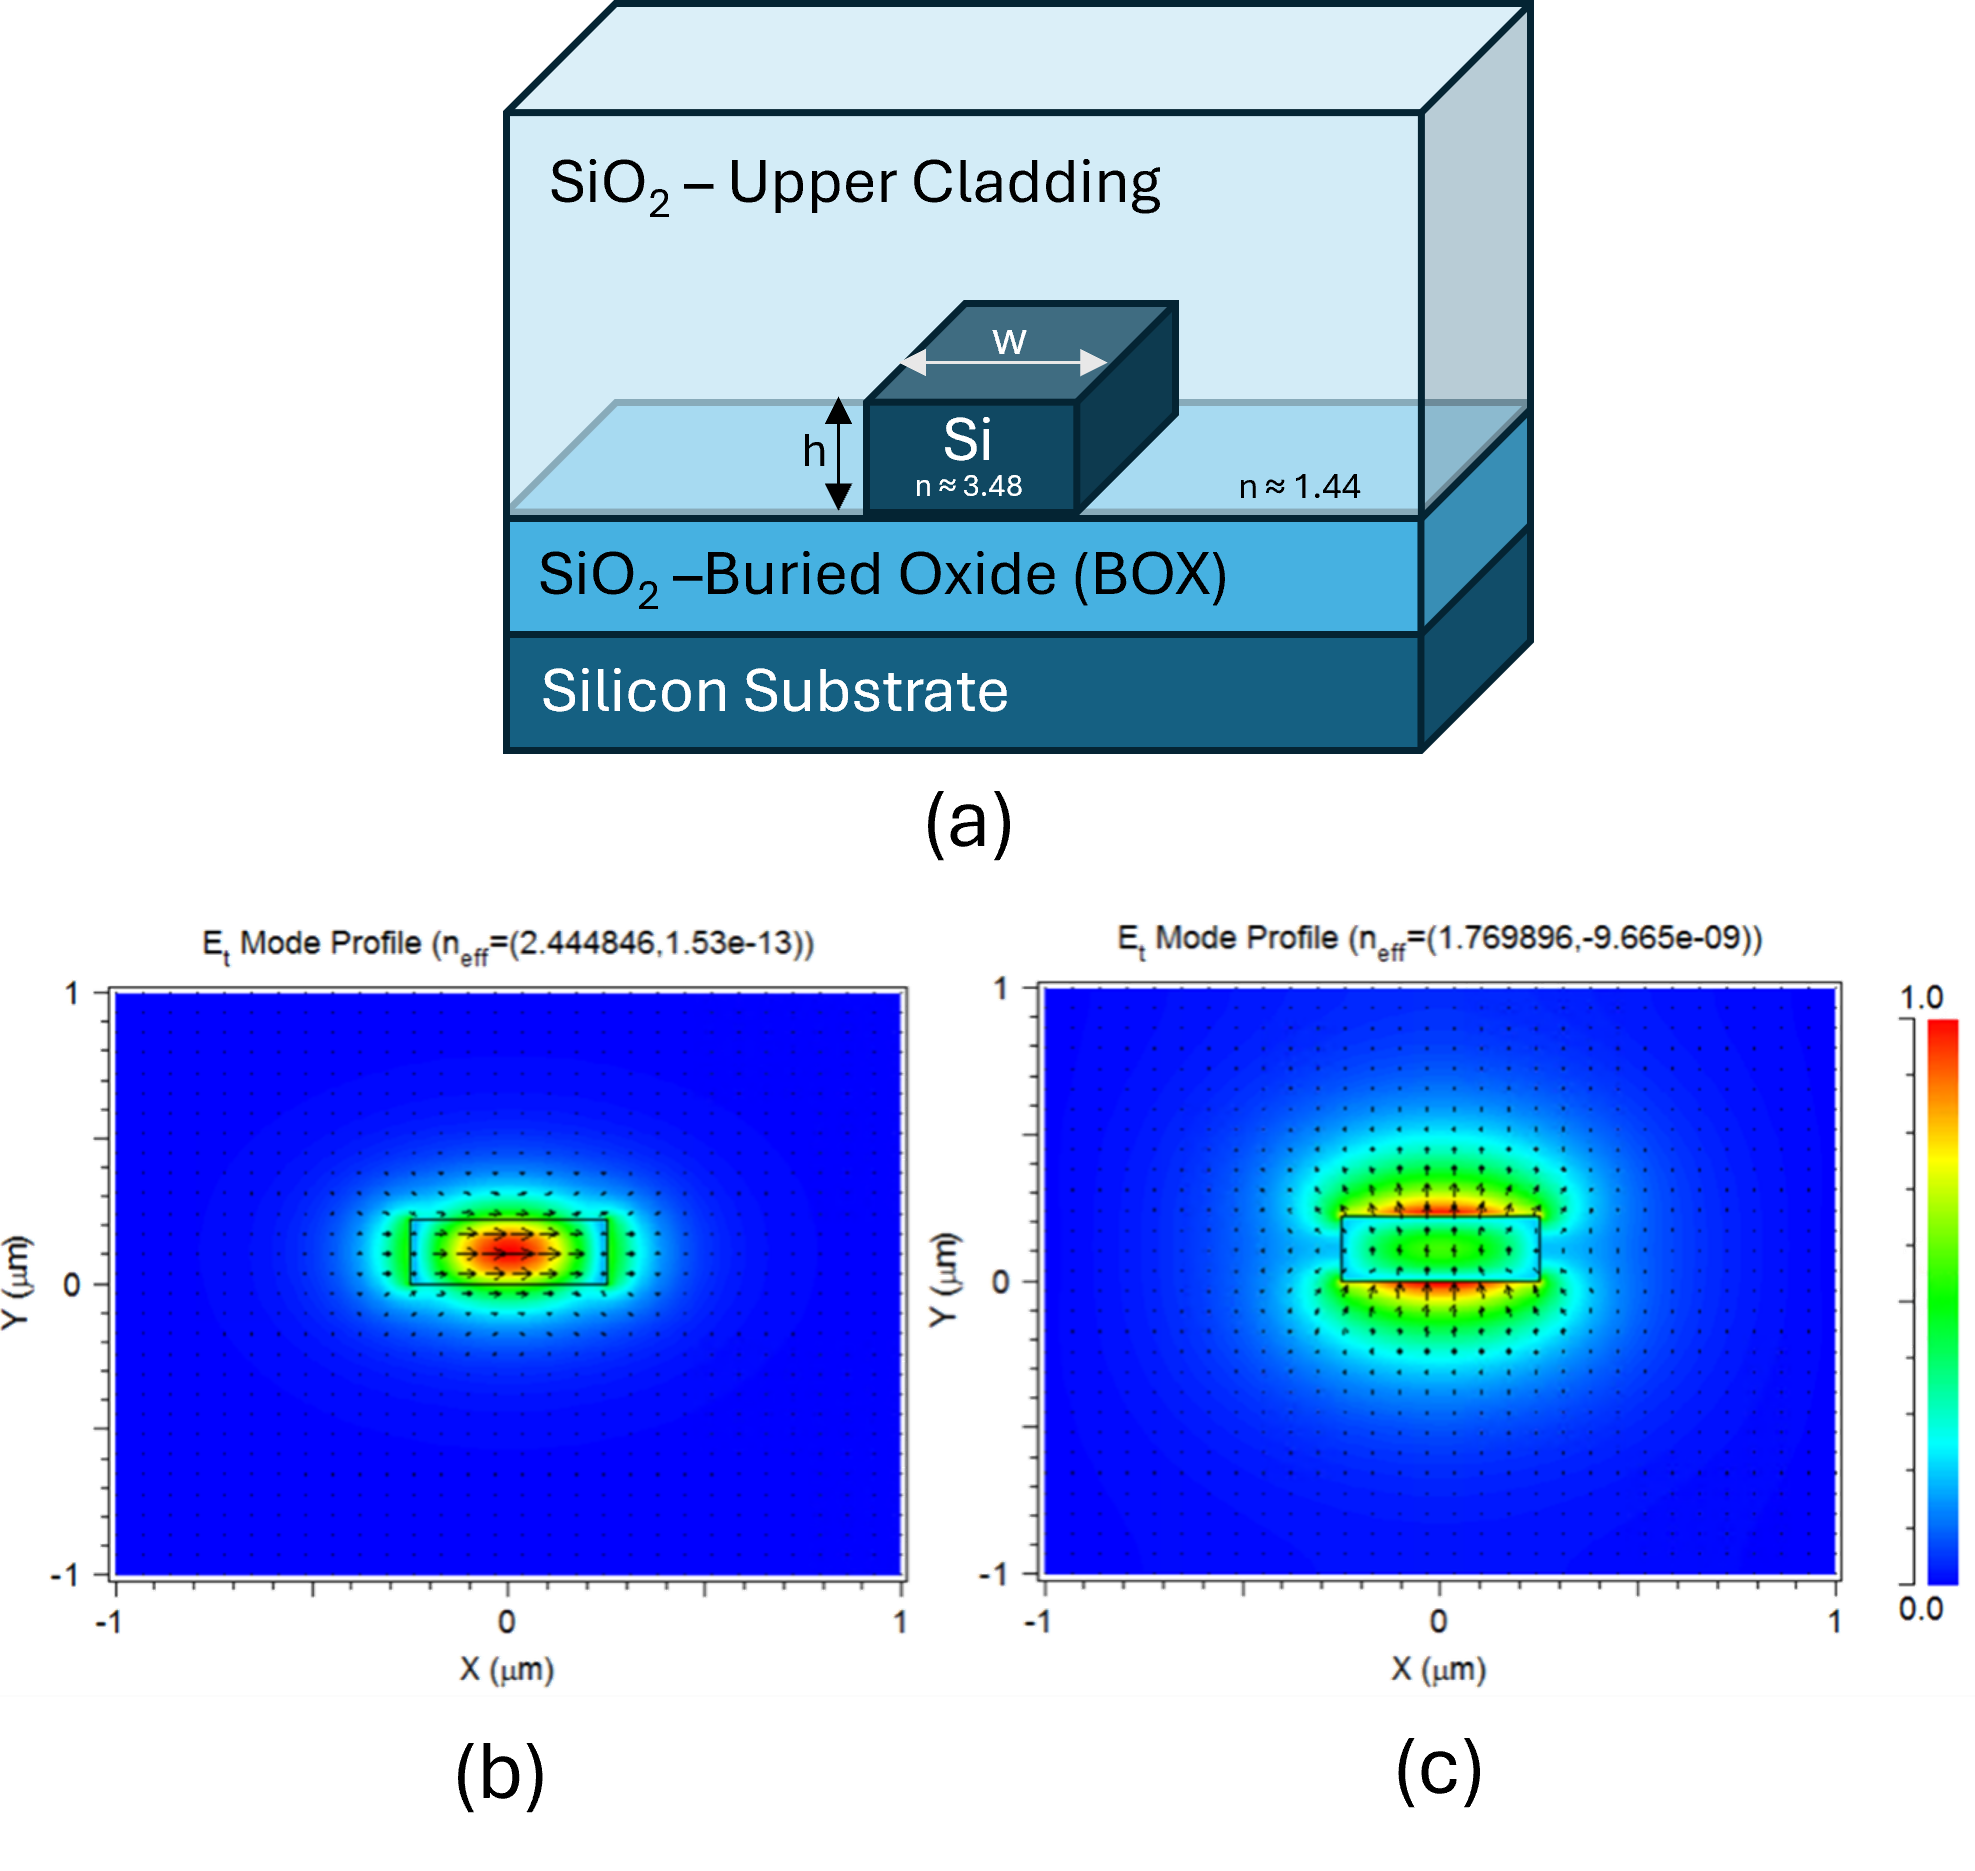
\includegraphics[width=0.7\linewidth]{figures/ch2-waveguide_modes.png}
    \caption{Standard-size silicon photonics waveguide. 
    (a) Cross-section of a generic SOI waveguide.
    (b) Simulation of fundamental TE guided mode. 
    (c) Simulation of fundamental TM guided mode.}
    \label{fig:ch2-waveguide_modes}
\end{figure}



The high confinement achievable in SOI waveguides enables compact interferometric and 
resonant devices, high integration density, and enhanced light-matter interaction. However, 
it also increases sensitivity to sidewall roughness and dimensional variations, making fabrication 
tolerances a critical design parameter. Small deviations in waveguide width or thickness can 
induce noticeable shifts in effective refractive index and device response.

Standard SOI photonic platforms are typically categorized according to device layer thickness. 
The most common configuration for telecommunications applications is the 220~nm silicon device 
layer, which supports single-mode operation for waveguide widths around 450–500~nm at 1550~nm. 
Thicker silicon layers (e.g., 300~nm or above) are also used in some processes to tailor modal 
confinement and improve performance in specific applications.

Thermal effects play a significant role in SOI-based devices due to the relatively large 
thermo-optic coefficient of silicon 
($\mathrm{d}n/\mathrm{d}T \approx 1.86 \times 10^{-4}~\mathrm{K}^{-1}$) 
\cite{cocorulloThermoopticalModulation15mm1992}. While this property enables efficient 
thermo-optic phase tuning, it also introduces thermal crosstalk and power consumption challenges 
in densely integrated circuits 
\cite{wattsAdiabaticThermoopticMach2013,coenenAnalysisThermalCrosstalk2022}.

Overall, the SOI platform provides a powerful combination of strong confinement, CMOS 
compatibility, and high integration density, which has positioned it as the dominant technology 
for large-scale silicon photonic circuits. These characteristics make SOI particularly well 
suited for the realization of complex circuits composed of multiple passive and active building 
blocks, which are discussed in the next section.



\section{Building Blocks of Programmable Circuits}

Programmable photonic circuits are constructed from a combination of passive optical structures 
and active tuning elements that, when properly interconnected, enable dynamic control over light 
propagation and interference. While passive components define the static topology of the circuit, 
active elements introduce the tunability required for reconfigurability.

The fundamental reconfigurable element in programmable photonic systems is the Programmable Unit 
Cell (PUC), which combines passive coupling structures with tunable phase shifters to implement a 
fully controllable 2x2 linear optical transformation. Before introducing the PUC in detail, it is 
necessary to review the passive and active building blocks from which it is constructed.

\subsection{Fundamental Passive Building Blocks}\label{sec:passive_bb}

Passive building blocks define the static optical backbone of programmable photonic circuits. They 
determine how light is distributed, combined, routed, and coupled within the chip. Although they 
do not provide tunability by themselves, they establish the interference pathways that, when 
combined with active phase control, enable full reconfigurability.

In silicon photonics, passive components are implemented using high-index-contrast waveguides in 
the Silicon-on-Insulator platform. The strong confinement provided by the refractive index 
contrast between silicon and silicon dioxide enables compact implementations of couplers, 
interferometers, crossings, and fiber-chip interfaces. However, this high confinement also 
increases sensitivity to fabrication variations, making precise design and modeling essential.

The most relevant passive building blocks for programmable circuits are directional couplers, 
multi-mode interferometers (MMIs), waveguide crossings, grating couplers, and edge couplers.

\subsubsection*{Directional Couplers}

Directional couplers are among the most fundamental passive elements in integrated photonics. 
They rely on evanescent coupling between two waveguides placed in close proximity over a finite 
interaction length. When the separation between the waveguides is sufficiently small, the 
evanescent tails of their guided modes overlap, enabling periodic power exchange.

The evolution of optical power along the coupling region can be described using coupled-mode 
theory. For identical waveguides, the power transferred from waveguide 1 to waveguide 2 after a 
propagation length $L$ is given by

\begin{equation}
P_2(L) = P_1(0)\sin^2(\kappa L),
\end{equation}

where $\kappa$ is the coupling coefficient, determined by the modal overlap and separation 
distance. The characteristic length required for complete power transfer, known as the coupling 
length, is

\begin{equation}
L_c = \frac{\pi}{2\kappa}.
\end{equation}

By selecting the appropriate interaction length $L$, directional couplers can implement arbitrary
fixed splitting ratios. In programmable photonic circuits, they are typically designed as balanced
50:50 couplers ($L = L_c/2$), forming the basis of interferometric structures such as Mach-Zehnder
interferometers.

Beyond power distribution, the operation of a symmetric directional coupler is more accurately 
described by its complex-valued transfer matrix $\mathbf{T}_{\text{DC}}$. This matrix relates the 
input complex field amplitudes $(E_{in,1}, E_{in,2})$ to the output amplitudes 
$(E_{out,1}, E_{out,2})$ as:

\begin{equation}
\begin{pmatrix} E_{out,1} \\ E_{out,2} \end{pmatrix} = \mathbf{T}_{\text{DC}} \begin{pmatrix} 
    E_{in,1} \\ E_{in,2} \end{pmatrix} = \begin{pmatrix} \cos(\kappa L) & -j\sin(\kappa L) \\ 
        -j\sin(\kappa L) & \cos(\kappa L) \end{pmatrix} \begin{pmatrix} E_{in,1} \\ E_{in,2} 
        \end{pmatrix}.
\label{eq:matrix_dc}
\end{equation}


For a perfectly balanced 3-dB coupler, the coupling term $\kappa L$ equals $\pi/4$, yielding a 
$\pi/2$ phase shift between the bar and cross ports. However, the performance of these components 
is highly sensitive to wavelength fluctuations and fabrication tolerances. Small stochastic 
deviations in waveguide width or gap separation modify the effective coupling coefficient 
($\kappa \pm \Delta\kappa$), resulting in an imbalanced or non-unitary matrix. In large-scale 
programmable architectures, these systematic errors propagate through the mesh, directly 
impacting the fidelity of the synthesized optical transformations 
\cite{chrostowskiSiliconPhotonicsDesign2015}.


\begin{figure}[h!]
    \centering
    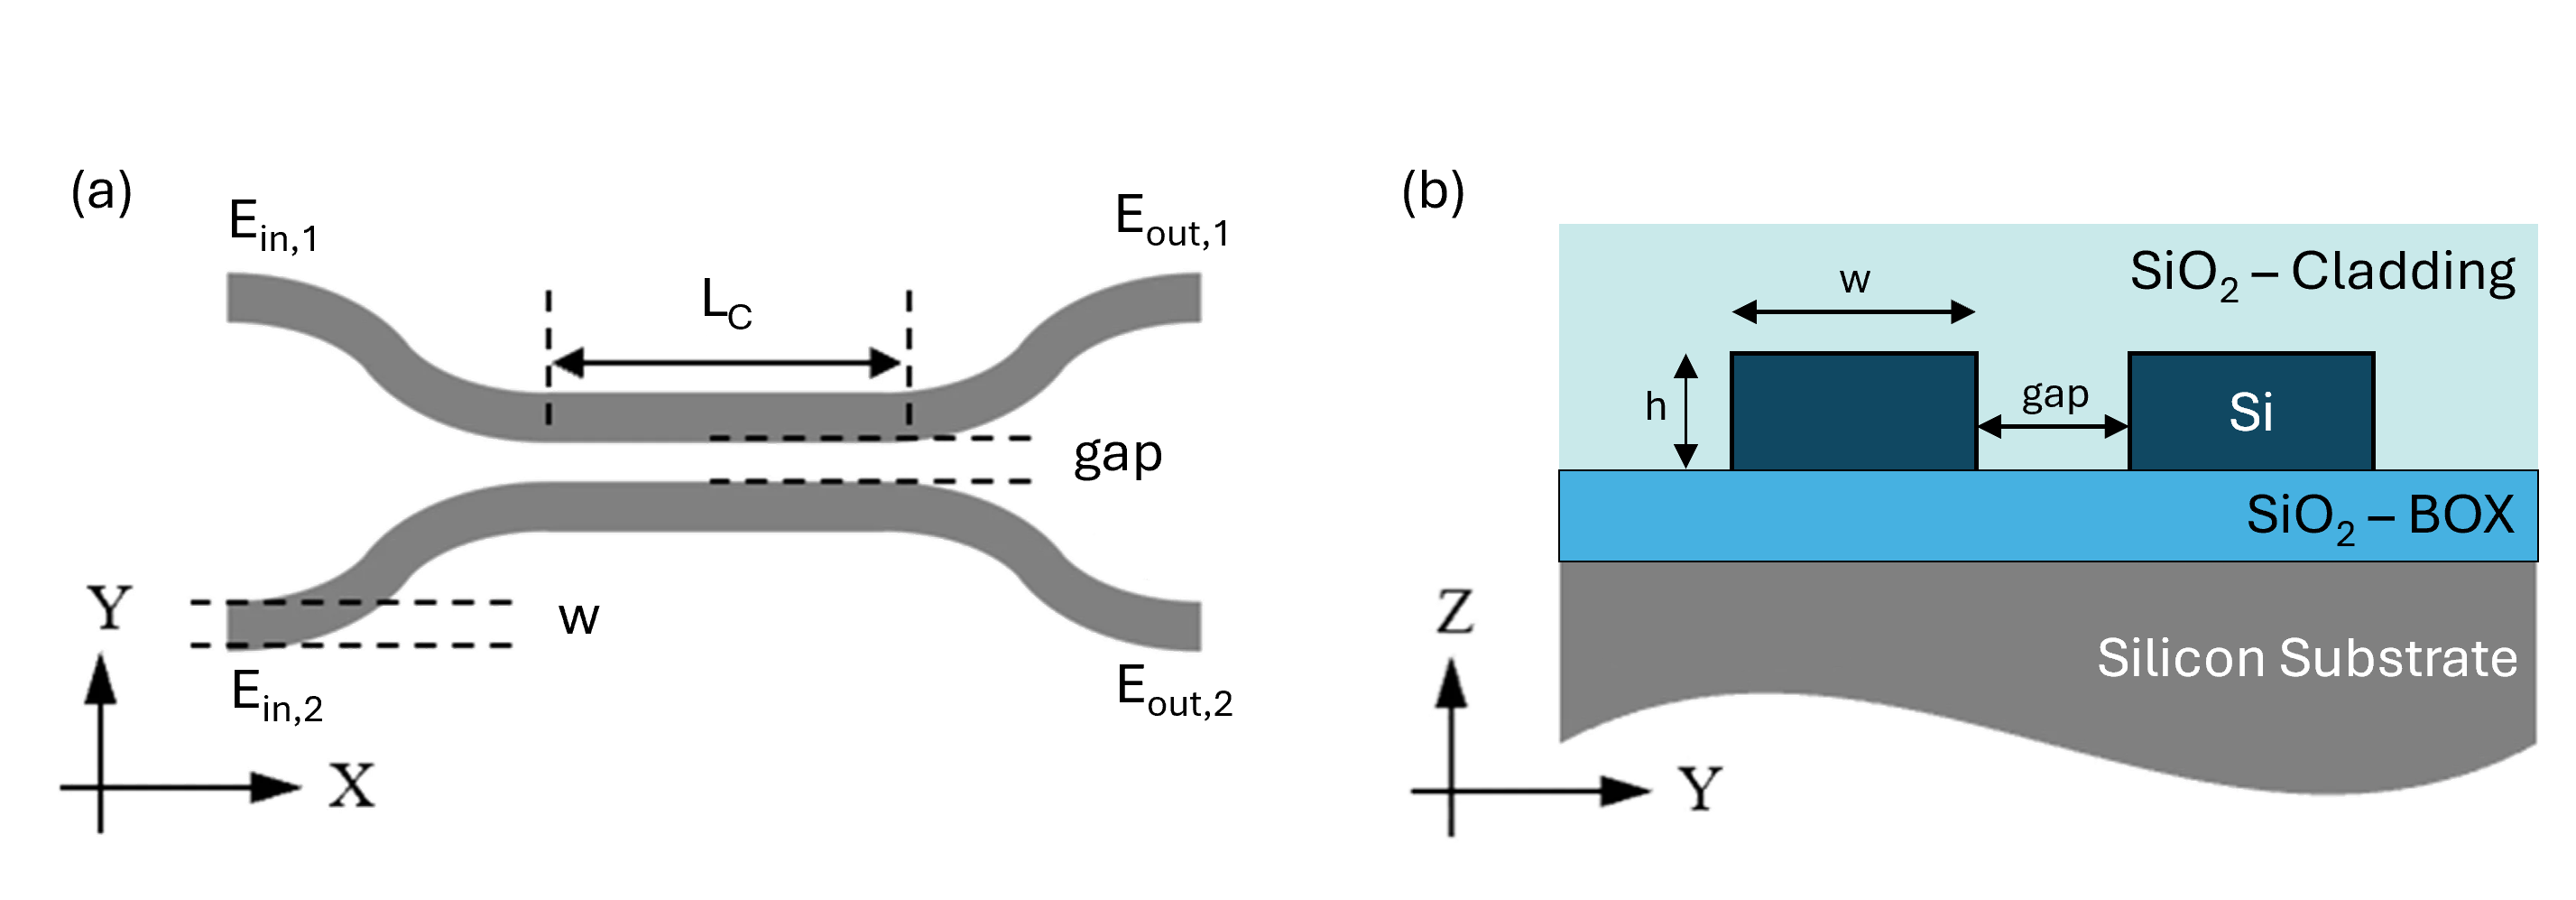
\includegraphics[width=\linewidth]{figures/ch2-directional_coupler.png}
    \caption{Schematic of a $2\times2$ symmetric directional coupler. 
    (a) Top-view illustrating the interaction length $L$ and the coupling gap. 
    (b) Cross-section of the coupling region in the SOI platform, where the waveguide width $w$ and 
    the gap are the critical parameters defining the coupling coefficient $\kappa$.}
\end{figure}



\subsubsection*{Multi-Mode Interferometers (MMIs)}

Multi-mode interferometers exploit the self-imaging principle in multimode waveguides. When light 
is injected into a multimode section, multiple transverse modes propagate with different 
propagation constants. The interference between these modes leads to periodic reproduction of the 
input field profile at specific distances along the propagation direction.

The characteristic beat length between the two lowest-order modes is given by

\begin{equation}
L_\pi = \frac{\pi}{\beta_0 - \beta_1},
\end{equation}

where $\beta_0$ and $\beta_1$ are the propagation constants of the fundamental and first-order 
modes, respectively. For an MMI operating in the restricted paired interference regime (where the 
input field is launched at $x = \pm W/6$), the length required to form a two-fold self-image (3-dB 
splitter) is significantly reduced and can be approximated as

\begin{equation}
L_{\text{MMI}} \approx \frac{L_\pi}{2}.
\end{equation}

The self-imaging mechanism in a $2\times2$ MMI results in a transfer matrix 
$\mathbf{T}_{\text{MMI}}$ that, assuming an ideal device with balanced splitting, is given by:

\begin{equation}
\mathbf{T}_{\text{MMI}} = \frac{1}{\sqrt{2}} \begin{pmatrix} 1 & e^{j\pi/2} \\ e^{j\pi/2} & 1 
\end{pmatrix} = \frac{1}{\sqrt{2}} \begin{pmatrix} 1 & j \\ j & 1 \end{pmatrix}.
\label{eq:matrix_mmi}
\end{equation}



To illustrate the self-imaging principle in a practical building block, Figure 
\ref{fig:ch2-mmi_2x2_self_imagin} shows a Beam Propagation Method (BPM) simulation of a $2\times2$ 
MMI designed for the paired interference regime. By launching the input field at a transverse 
position of $x = \pm W/6$, the device can function as either a balanced power splitter or a 
cross-coupler depending on its longitudinal dimension.

As observed in the simulation, at a distance of approximately $L_{\pi}/2$, the interference of the 
excited modes generates two symmetric images of the input field, realizing a 3-dB splitting ratio. 
Further propagation to $z \approx L_{\pi}$ results in a single reconstructed image at the opposite 
(cross) output port. It is worth noting that in high-index-contrast platforms like SOI, numerical 
calibration is essential to account for the effective width expansion due to field penetration into 
the cladding. From a fault-tolerance perspective, the stability of these imaging points against 
small lithographic deviations in $W$ is what makes the MMI a more reliable candidate than 
directional couplers for the backbone of large-scale programmable meshes.

\begin{figure}[!ht]
    \centering
    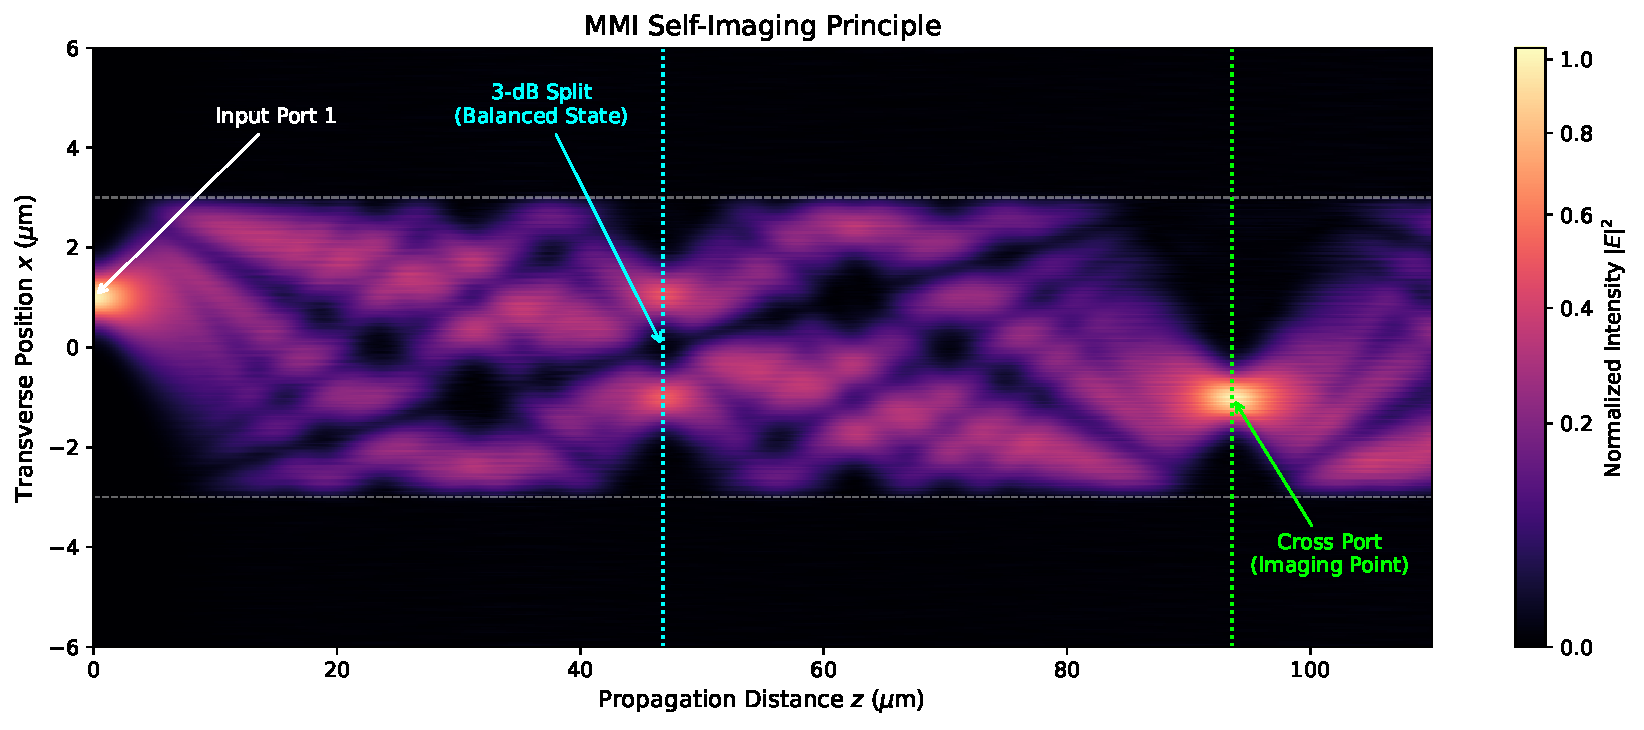
\includegraphics[width=\textwidth]{figures/ch2-mmi_2x2_self_imagin.pdf}
    \caption{BPM simulation of a $2\times2$ MMI. Vertical markers indicate the numerically 
    calibrated 3-dB splitting ($L_{\pi}/2$) and cross-over ($L_{\pi}$) imaging planes.}
    \label{fig:ch2-mmi_2x2_self_imagin}
\end{figure}

In the context of large-scale integration, MMIs offer a significant advantage in terms of 
\textit{fault tolerance} compared to directional couplers. Their performance is primarily 
determined by the width of the multimode interference region; since $W_e$ is typically several 
micrometers wide, nanometric lithographic variations represent a much smaller relative error than 
in the narrow gaps of directional couplers. Consequently, MMIs exhibit superior robustness against 
fabrication tolerances and wavelength fluctuations, ensuring a more stable power splitting ratio 
(lower imbalance) across the chip \cite{soldanoOpticalMultimodeInterference1995}. While they 
require a larger footprint and may introduce slightly higher insertion losses due to mode mismatch 
at the junctions, their reliability makes them the preferred choice for the static backbone of 
programmable photonic meshes.

\FloatBarrier



\subsubsection*{Waveguide Crossings}

Waveguide crossings are essential for enabling complex optical routing in two-dimensional layouts, 
allowing waveguides to intersect without the need for additional lithographic layers. In 
large-scale programmable meshes, where dense interconnections and mesh-like topologies are 
required, the performance of these crossings becomes a critical factor for scalability.

A simple orthogonal intersection of two single-mode waveguides introduces significant scattering 
losses and crosstalk (typically ranging from $-20$ to $-30$ dB) due to the modal mismatch and 
radiation at the intersection region. To mitigate these effects, advanced crossing designs—such as 
those based on parabolic tapers, Bloch-mode engineering, or Multi-Mode Interference regions—are 
employed to expand the mode and minimize field intensity at the waveguide boundaries during the 
transition.

The impact of a crossing can be modeled by its transfer matrix $\mathbf{T}_{\text{cross}}$, 
relating the throughput and the leaked (crosstalk) signals:
\begin{equation}
\begin{pmatrix} E_{out,1} \\ E_{out,2} \end{pmatrix} = \mathbf{T}_{\text{cross}} \begin{pmatrix} 
    E_{in,1} \\ E_{in,2} \end{pmatrix} = \begin{pmatrix} \tau & j\sqrt{\chi} \\ j\sqrt{\chi} & \tau 
    \end{pmatrix} \begin{pmatrix} E_{in,1} \\ E_{in,2} \end{pmatrix},
\label{eq:matrix_crossing}
\end{equation}
where $\tau$ is the complex transmission coefficient (representing insertion loss) and $\chi$ is 
the power crosstalk coefficient. 

In the context of large-scale programmable circuits, even small crossing losses ($<0.1$ dB) 
accumulate over multiple stages, directly impacting the total power budget. Furthermore, the 
coherent accumulation of crosstalk from hundreds of crossings acts as a noise floor that 
interferes with the intended signal, limiting the extinction ratio and the precision of the 
synthesized optical transformations. Therefore, ultra-low-loss and low-crosstalk crossings are 
paramount for maintaining signal fidelity in deep interferometric networks.


To address the scalability limits imposed by conventional intersections, advanced designs such as 
the one proposed by Ding et al. \cite{maUltralowLossSingle2013} are employed. As illustrated in 
Figure \ref{fig:ch2-crossing_Ding_adapted}, this geometry utilizes optimized spline-based tapers to 
adiabatically expand the guided mode before the intersection. By increasing the mode field diameter, 
the optical intensity at the waveguide corners is significantly reduced, which suppresses 
scattering and minimizes crosstalk to levels below $-37$ dB with insertion losses as low as $0.028$ 
dB. Such high-performance characteristics are fundamental for the fault-tolerant operation of 
large-scale meshes, ensuring that the cumulative noise floor remains below critical thresholds for 
optical signal processing.

\begin{figure}[htbp]
    \centering
    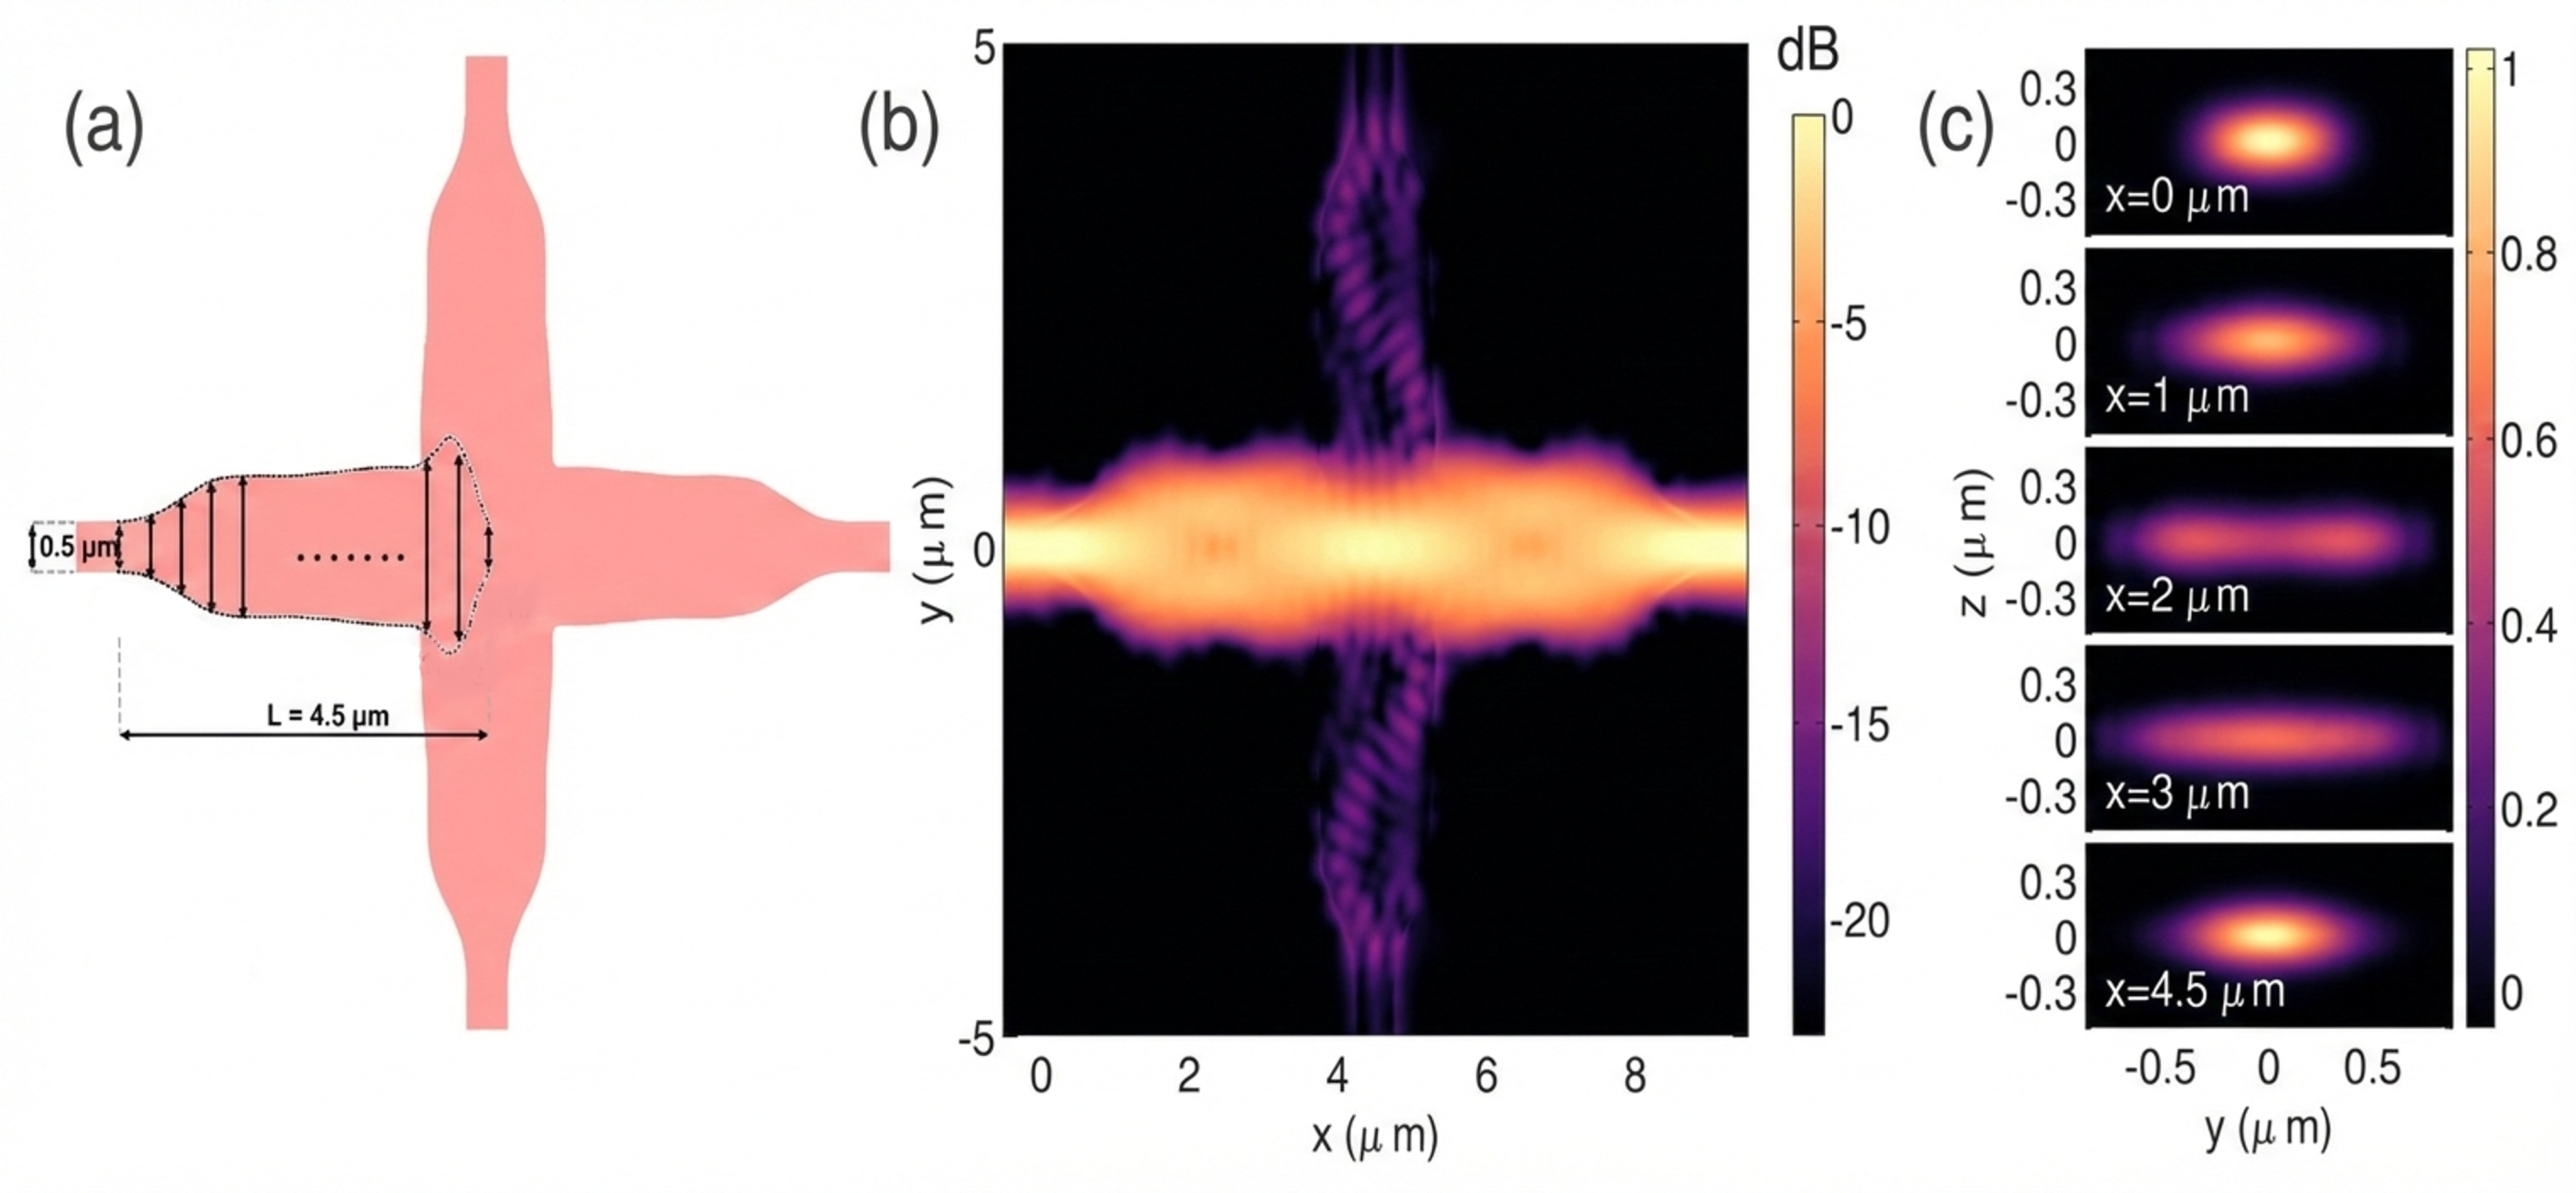
\includegraphics[width=\textwidth]{figures/ch2-crossing_Ding_adapted} 
    \caption{Optimized silicon waveguide crossing design. 
    (a) Layout geometry using spline-based tapers, 
    (b) electric field intensity simulation, and 
    (c) transverse mode profiles at different stages of the crossing. 
    Adapted from Ding et al. \cite{maUltralowLossSingle2013}.}
    \label{fig:ch2-crossing_Ding_adapted}
\end{figure}


\subsubsection*{Grating Couplers}

Grating couplers provide a practical solution for out-of-plane coupling between single-mode optical 
fibers and planar waveguides. They operate based on the diffraction from a periodic perturbation in 
the waveguide, enabling phase matching between the guided mode and an externally incident fiber 
mode. 

As illustrated in Figure \ref{fig:ch2-grating}, the fiber is typically positioned at a 
tilt angle $\theta$ (usually $8^\circ$ to $10^\circ$) relative to the surface normal to prevent 
second-order reflections back into the fiber. The grating period $\Lambda$ must satisfy the 
phase-matching condition:

\begin{equation}
\Lambda = \frac{\lambda}{n_{\text{eff}} - n_{\text{clad}}\sin\theta},
\label{eq:grating_period}
\end{equation}

where $\lambda$ is the operating wavelength, $n_{\text{eff}}$ is the effective index of the guided 
mode, and $n_{\text{clad}}$ is the refractive index of the cladding material.

\begin{figure}[!ht]
    \centering
    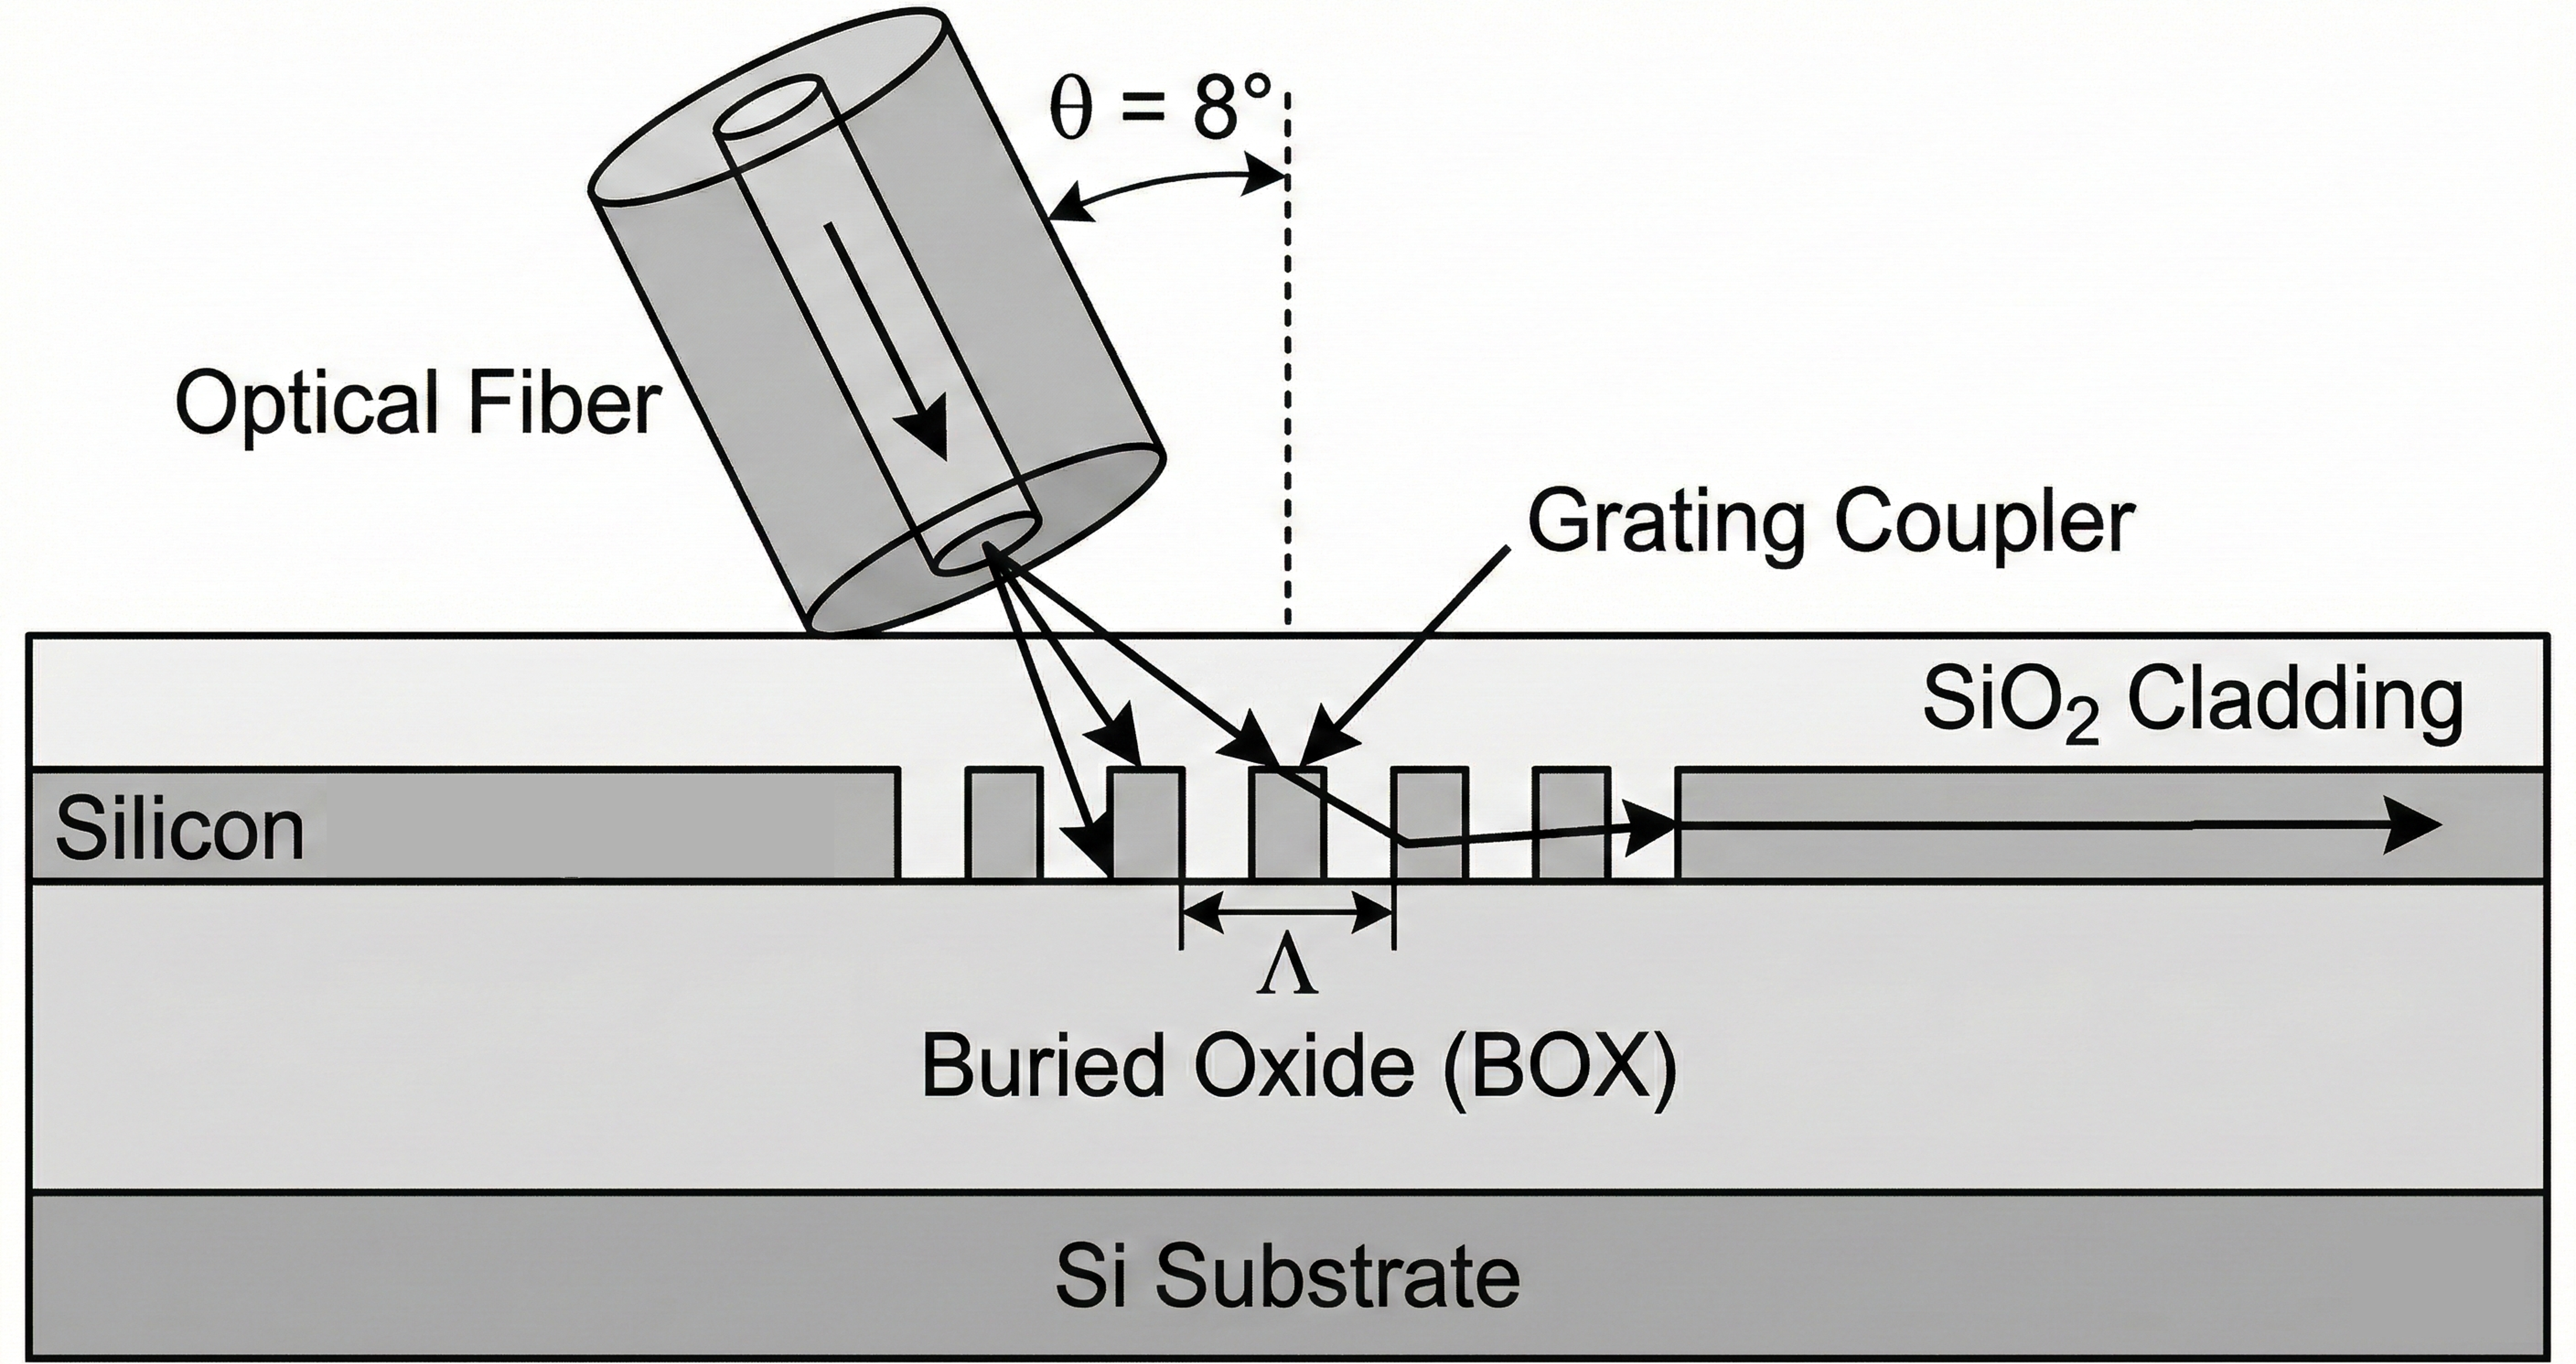
\includegraphics[width=0.7\textwidth]{figures/ch2-grating}
    \caption{Schematic cross-section of a Silicon-on-Insulator grating coupler. The diagram 
    illustrates the diffraction of light from a tilted single-mode fiber into the silicon waveguide 
    core. Key parameters such as the grating period $\Lambda$, the tilt angle $\theta$, and the 
    layer stack (Cladding, BOX, and Substrate) are indicated.}
    \label{fig:ch2-grating}
\end{figure}

\FloatBarrier

Grating couplers are highly advantageous for large-scale integration as they enable wafer-scale 
testing without the need for dicing or facet polishing. However, they typically introduce higher 
insertion losses ($3$--$5$ \text{dB}) and have a limited operational bandwidth compared to edge 
coupling techniques. Their efficiency and spectral response are highly sensitive to fabrication 
parameters such as the etch depth and the duty cycle of the grating teeth.


\subsubsection*{Edge Couplers}


Edge couplers, also known as Spot-Size Converters (SSCs), facilitate in-plane coupling between the 
optical fibers and the photonic chip. In the SOI platform, the high refractive index contrast leads 
to extremely high mode confinement within the silicon waveguides (typically with sub-micrometer 
dimensions of $500 \times 220$ nm). This presents a significant challenge for direct coupling, as 
standard single-mode fibers (SMF-28) exhibit a Mode Field Diameter (MFD) of approximately 
$10 \ \mu$m. The vast mismatch between these two mode sizes would result in prohibitive insertion 
losses without a dedicated transformation mechanism.

To bridge this gap, edge couplers utilize adiabatic tapers that gradually transition the mode from 
the high-confinement silicon core to a larger area that better matches the MFD of an external 
lensed fiber or an ultra-high numerical aperture (UHNA) fiber, which typically provide MFDs in the 
range of $2$ to $3 \ \mu$m. 

As illustrated in Figure \ref{fig:ch2-edge_coupler_info}a, this transition is typically realized 
through an inverted taper geometry. By gradually decreasing the silicon core width towards the chip 
facet, the structure facilitates the adiabatic expansion of the optical mode, preparing it for the 
interface with the external medium.

\begin{figure}[!ht]
    \centering
    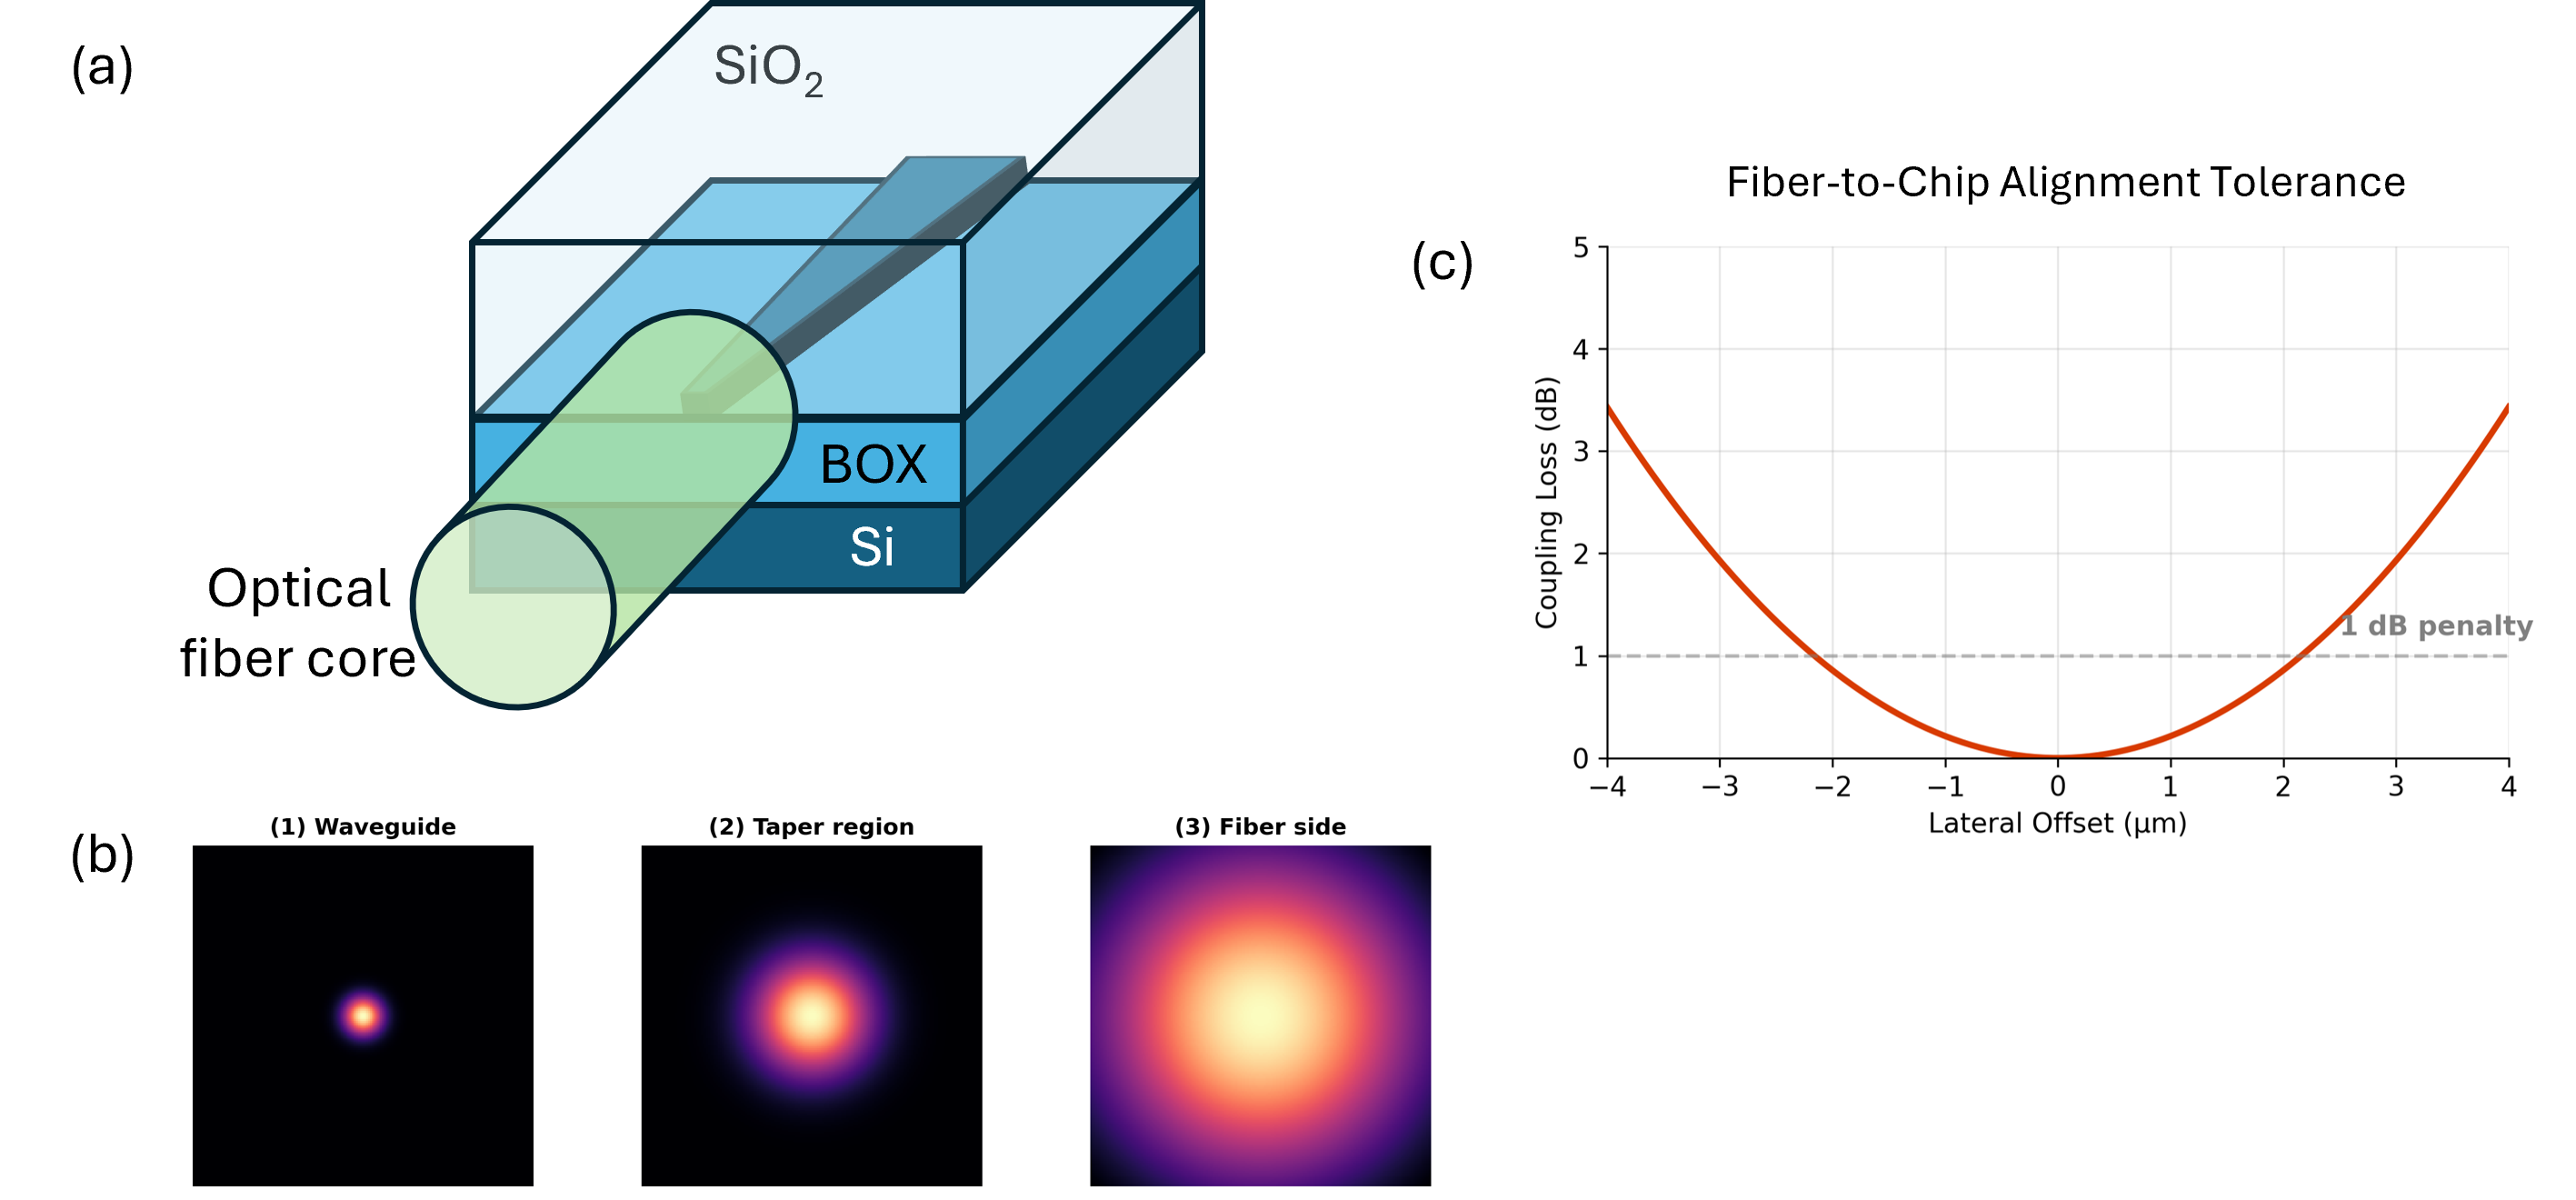
\includegraphics[width=\textwidth]{figures/ch2-edge_coupler_info}
    \caption{Edge coupler analysis: (a) 3D perspective of the inverse adiabatic taper embedded in a 
    low-index cladding. (b) $|E|^2$ mode field profiles showing the expansion of the optical mode 
    as the silicon core width decreases. (c) Calculated coupling loss as a function of lateral 
    fiber offset, illustrating the alignment tolerance of the interface.}
    \label{fig:ch2-edge_coupler_info}
\end{figure}

\FloatBarrier

The physical principle behind this transition is the reduction of the modal confinement. As 
evidenced by the mode profiles in Figure \ref{fig:ch2-edge_coupler_info}b, the narrow silicon tip 
forces the field to delocalize into the cladding, effectively matching the spot size of the 
external fiber. Unlike grating couplers, edge couplers are non-resonant devices, which grants them 
a significantly broader operational bandwidth and superior power efficiency, with insertion losses 
typically remaining below $1$~dB per facet. 
However, the efficiency of this coupling is highly sensitive to the mechanical positioning of the 
fiber. Figure \ref{fig:ch2-edge_coupler_info}c shows the impact of lateral misalignment on the total 
coupling loss. In the context of large-scale programmable meshes, these losses contribute to the 
overall power budget and can be a source of systematic error if the packaging process exhibits 
variations. Achieving sub-micrometer alignment remains a critical requirement for maintaining 
high-fidelity optical transformations across the circuit.


~ \\
% Closing of section 2.3.1 - Fundamental Passive Building Blocks 
The passive building blocks described above define the structural and interferometric framework of 
programmable photonic circuits. While these components do not provide tunability by themselves, 
they establish the essential coupling and interference pathways required to implement linear 
optical transformations.

When combining waveguides, splitters and combiners with active phase tuning elements, these 
structures form reconfigurable interferometric units capable of realizing arbitrary $2 \times 2$ 
transformations. The integration of these passive and active components culminates in the 
definition of the \textit{Programmable Unit Cell} (PUC), the fundamental building block of the 
mesh. This core element will be introduced in detail after discussing the physical mechanisms 
enabling dynamic phase control in the following section.



\subsection{Active Tuning Mechanisms}

Active tuning mechanisms provide the dynamic control required for programmable photonic operation.
 While passive structures define fixed coupling and interference pathways, active elements enable 
 external electrical control over the effective refractive index ($n_{\text{eff}}$) or the 
 absorption coefficient ($\alpha$) of guided modes. By inducing controlled phase shifts within 
 interferometric structures, these mechanisms allow the realization of arbitrary linear optical 
 transformations.

In silicon photonics, tunability is primarily achieved by exploiting physical effects that modify 
the refractive index of silicon. The most relevant approaches are based on the thermo-optic effect 
and the plasma dispersion effect, each offering different trade-offs in terms of speed, power 
consumption, and optical loss.



\subsubsection*{Thermo-Optic Phase Shifters}

The thermo-optic (T-O) effect is the most widely adopted tuning mechanism in silicon photonics due 
to its high efficiency, relatively simple fabrication, and compatibility with standard CMOS 
processes. Silicon exhibits a large thermo-optic coefficient:

\begin{equation}
\frac{dn}{dT} \approx 1.86 \times 10^{-4} \ \text{K}^{-1},
\end{equation}

which enables efficient phase modulation through local heating. By integrating a resistive 
micro-heater (typically made of TiN, NiCr, or Tungsten) above the waveguide cladding, the 
temperature of the silicon core can be precisely controlled. The induced phase shift $\Delta \phi$ 
over a length $L$ is given by:

\begin{equation}
\Delta \phi = \frac{2\pi}{\lambda} \frac{dn}{dT} \Delta T L,
\label{eq:thermo_phase}
\end{equation}

where $\Delta T$ represents the local temperature increase and $\lambda$ is the operating 
wavelength.

\begin{figure}[htbp]
    \centering
    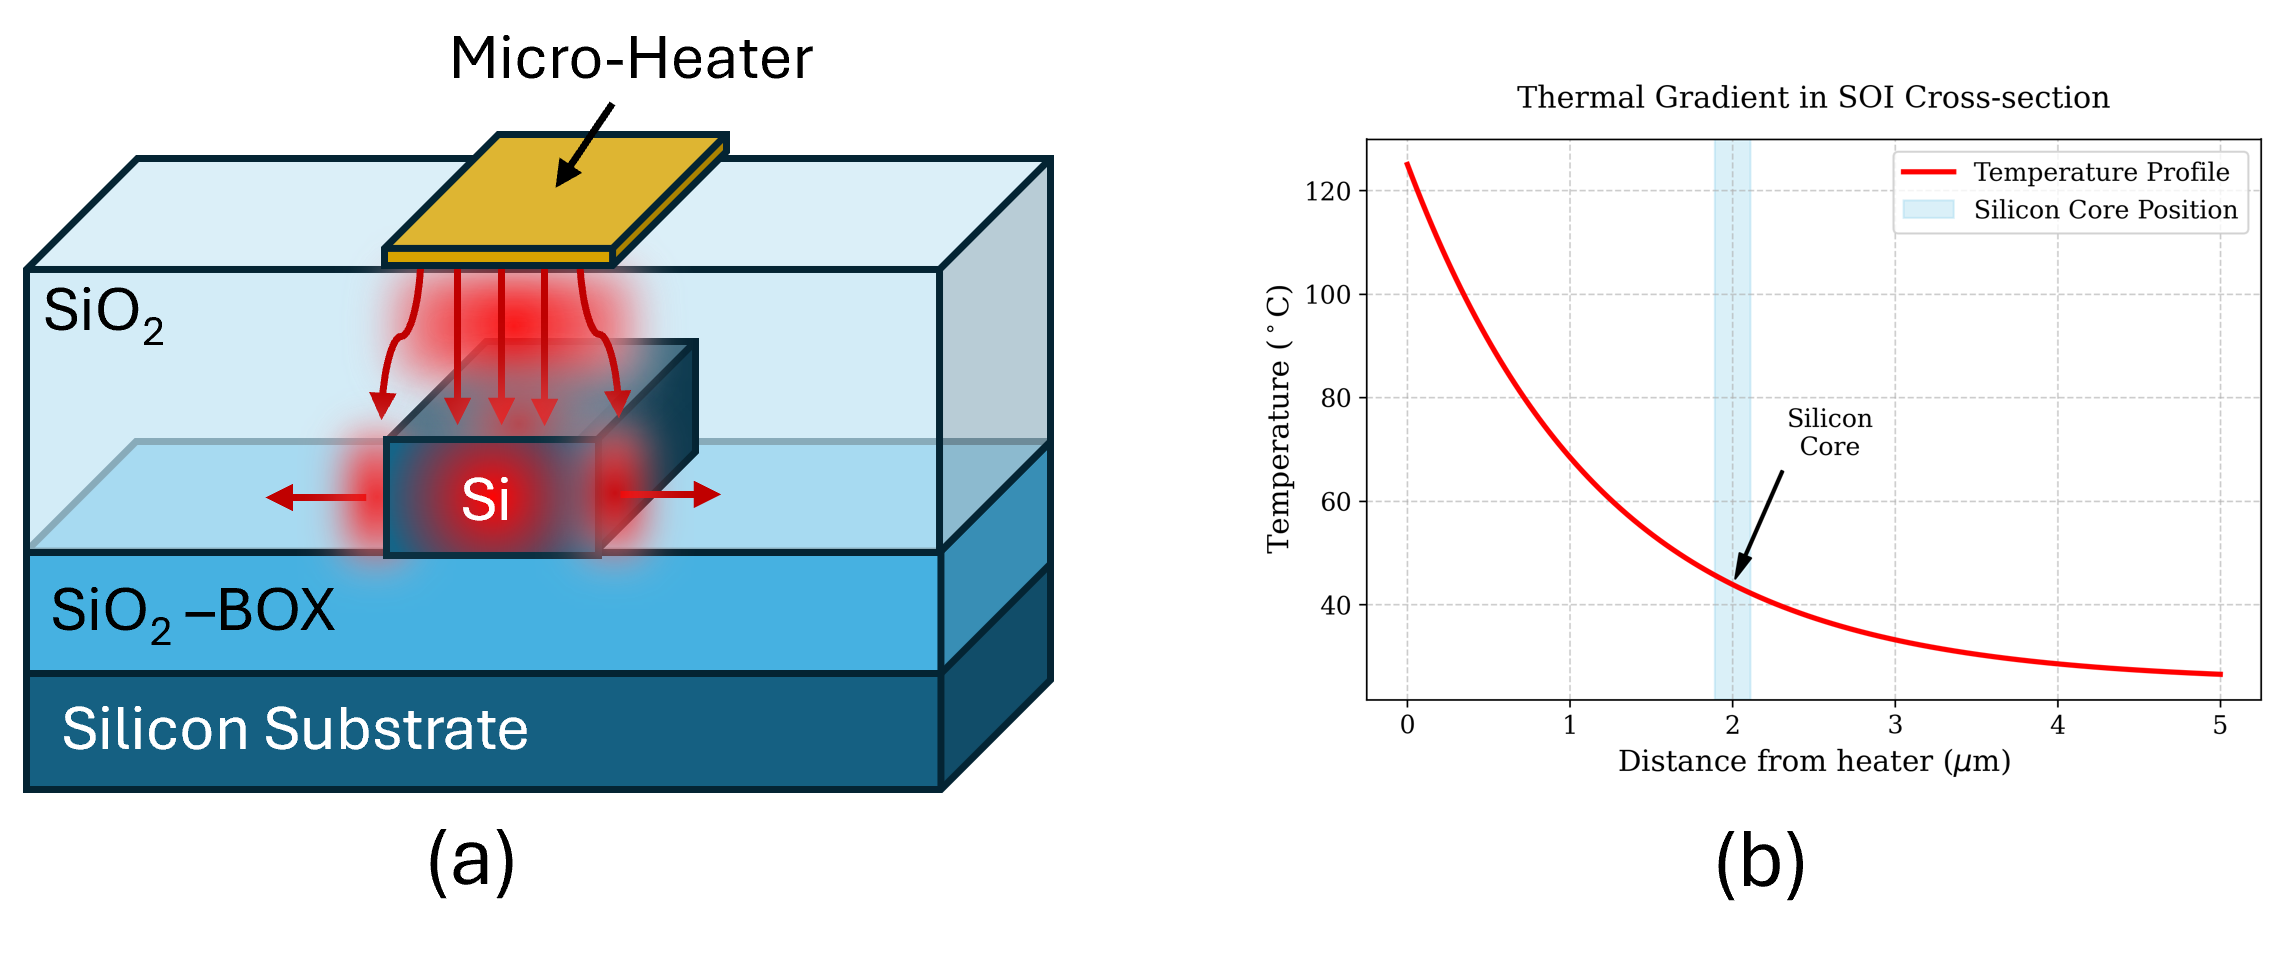
\includegraphics[width=0.9\textwidth]{figures/ch2-tops}
    \caption{Thermo-optic phase shifter (TOPS) analysis: (a) Cross-sectional schematic of an SOI 
    waveguide showing the micro-heater and the heat diffusion paths. (b) Simulated vertical 
    temperature profile from the heater surface towards the substrate, highlighting the thermal 
    gradient reaching the silicon core.}
    \label{fig:ch2-tops}
\end{figure}


The physical arrangement and the resulting thermal distribution are illustrated in Figure 
\ref{fig:ch2-tops}. As shown in the cross-section (Fig. \ref{fig:ch2-tops}a), the heat generated by 
the metallic element must diffuse through the upper cladding to reach the waveguide core. The 
simulated temperature gradient in Fig. \ref{fig:ch2-tops}b demonstrates that while the silicon core 
reaches the necessary $\Delta T$ for phase shifting, a significant amount of heat also spreads 
laterally.

While TOPS offer a large tuning range and negligible additional propagation loss, this lateral heat 
spread leads to thermal crosstalk, where the operation of one heater inadvertently affects 
neighboring interferometers. Furthermore, the mechanism is limited by the thermal diffusion time 
constant, resulting in millisecond-scale response times ($\tau \approx 10$--$100 \ \mu\text{s}$). 
In large-scale programmable meshes, managing these thermal effects is a critical challenge that 
requires specialized isolation structures or compensation algorithms 
\cite{bogaertsProgrammablePhotonicCircuits2020}.

\FloatBarrier


\subsubsection*{Carrier-Based Phase Shifters}

For applications requiring high-speed reconfiguration, the plasma dispersion effect is employed.
Variations in the free carrier concentration modify both the real part of the refractive index and 
the absorption coefficient of silicon. According to the empirical relations provided by Soref and 
Bennett \cite{sorefElectroopticalEffectsSilicon1987}, the variations at $\lambda = 1550$ nm are:

\begin{equation}
\Delta n = - [8.8 \times 10^{-22} \Delta N_e + 8.5 \times 10^{-18} (\Delta N_h)^{0.8}]
\end{equation}
\begin{equation}
\Delta \alpha \ [\text{cm}^{-1}] = 8.5 \times 10^{-18} \Delta N_e + 6.0 \times 10^{-18} \Delta N_h
\end{equation}

where $\Delta N_e$ and $\Delta N_h$ are the changes in electron and hole concentrations 
(in $\text{cm}^{-3}$), respectively. 

\begin{figure}[htbp]
    \centering
    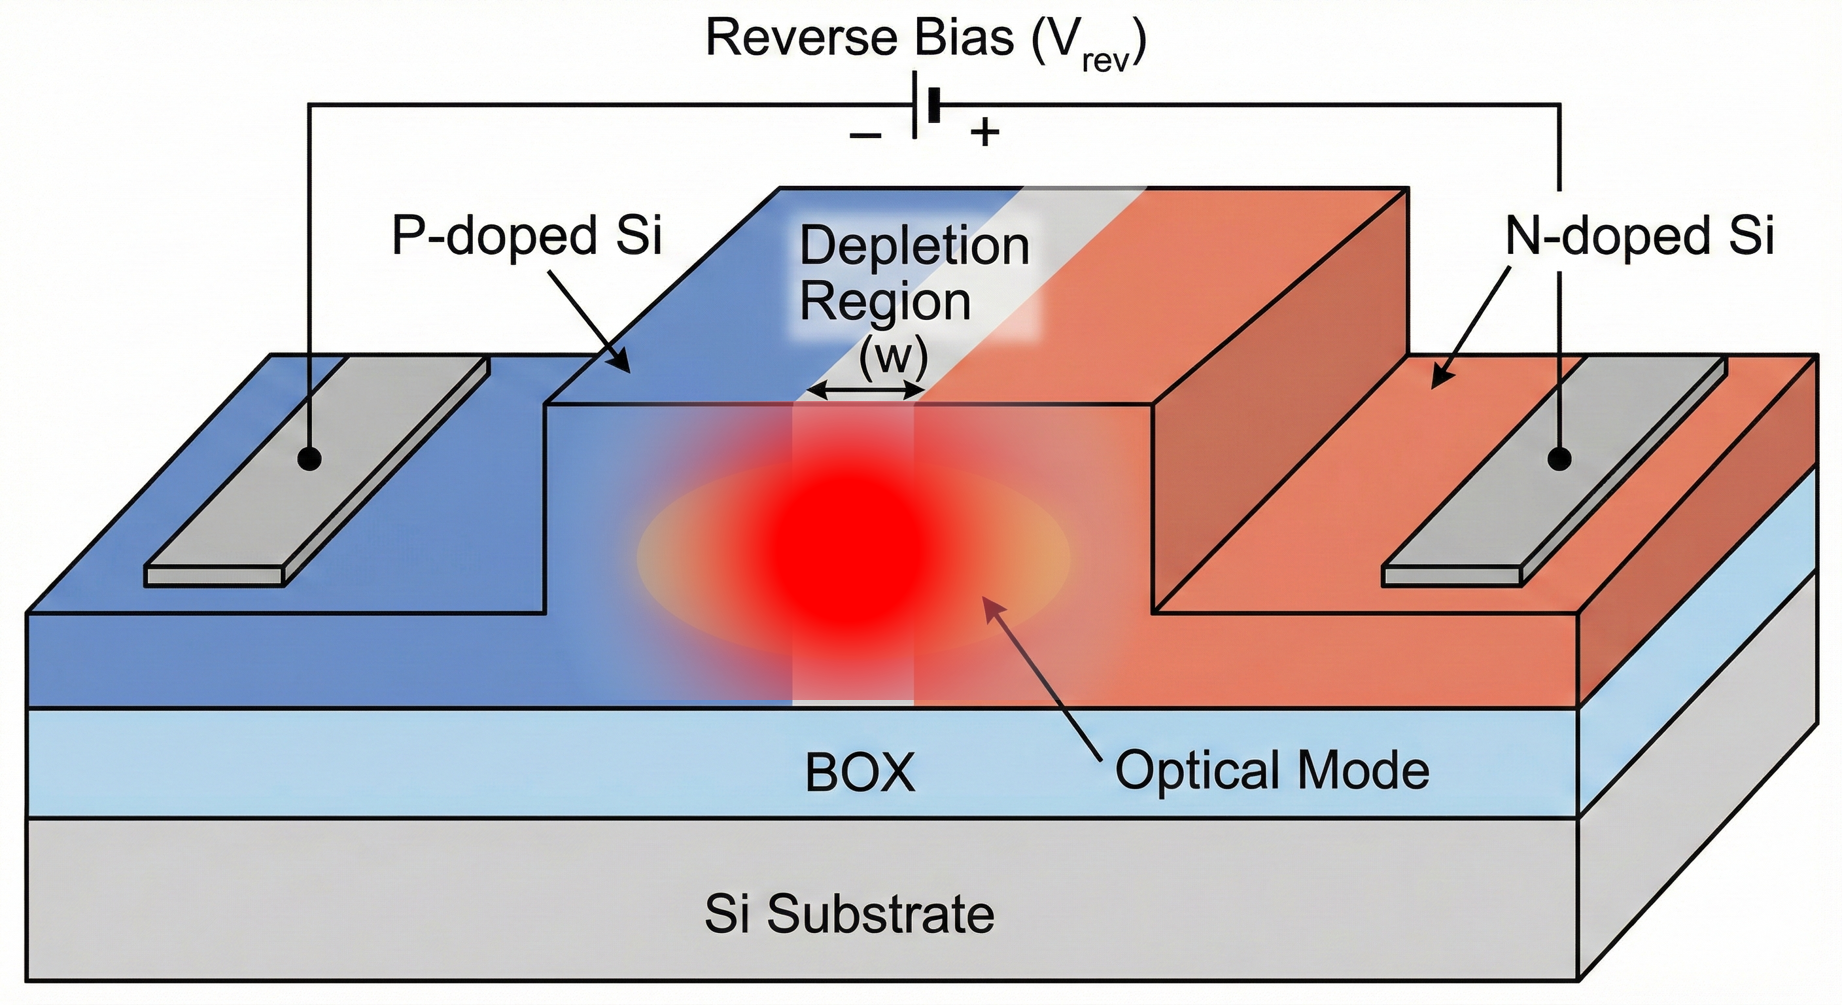
\includegraphics[width=0.6\textwidth]{figures/ch2-pn_doped_si}
    \caption{Schematic of a lateral PN junction integrated within a silicon rib waveguide. The 
    modulation of the depletion region width under reverse bias enables high-speed phase control.}
    \label{fig:h2-pn_doped_si}
\end{figure}

\FloatBarrier

Carrier-based phase shifters are typically implemented using PN or PIN junctions 
\cite{reedSiliconOpticalModulators2010}. While they offer modulation speeds up to tens of GHz, they 
introduce intrinsic electro-optical trade-offs: carrier injection provides high efficiency but 
limited speed and high loss, while carrier depletion offers ultra-fast operation with lower 
efficiency.

\subsubsection*{Performance Trade-Offs and Scalability}

The choice of tuning mechanism directly impacts the scalability of programmable photonic circuits. 
Table \ref{tab:tuning_comparison} summarizes the key performance metrics for the discussed 
mechanisms.

\begin{table}[htbp]
\centering
\caption{Comparison of active tuning mechanisms in SOI.}
\label{tab:tuning_comparison}
\begin{tabular}{l c c c}
\hline
\textbf{Feature} & \textbf{Thermo-Optic} & \textbf{Carrier Depletion} & \textbf{Carrier Injection} \\ \hline
Response Time & $\sim \mu\text{s}$ to ms & $\sim \text{ps}$ & $\sim \text{ns}$ \\
Added Optical Loss & Negligible & Moderate & High \\
Power Consumption & High (Static) & Ultra-low & Moderate \\
Scalability & High (Thermal limited) & High (Loss limited) & Moderate \\ \hline
\end{tabular}
\end{table}

In practical implementations, the integration of these active elements with the passive structures 
discussed in Section \ref{sec:passive_bb} culminates in the definition of the 
\textit{Programmable Unit Cell} (PUC). The PUC acts as the fundamental building block of the mesh, 
enabling the synthesis of arbitrary $2 \times 2$ unitary transformations through the coordinated 
control of phase and coupling.



\section{The Programmable Unit Cell (PUC)}
\label{sec:ch2-puc}

The Programmable Unit Cell (PUC) constitutes the fundamental building block of large-scale 
software-defined photonic integrated circuits. While several topologies exist, the most widely 
adopted architecture is based on the Mach-Zehnder Interferometer (MZI), which allows for the 
continuous manipulation of optical signals through controlled interference.

\subsection{Symmetric MZI Architecture}

In this work, the PUC is implemented as a balanced, symmetric MZI consisting of two $3$-dB 
couplers and active phase shifters integrated into both internal arms, as illustrated in 
Figure \ref{fig:ch2-puc}a. This dual-drive configuration, consistent with established 
programmable photonics standards \cite{capmanyProgrammableIntegratedPhotonics2020}, provides 
enhanced control over the interference conditions and improves the overall thermal stability of the 
device.

The operational state of the cell is governed by the phase induced in the upper arm ($\phi_{upper}$) 
and the lower arm ($\phi_{lower}$). For the characterization of the cell's response, we define the 
differential phase shift as:

\begin{equation}
\Delta\phi = \phi_{upper} - \phi_{lower}
\label{eq:delta_phi}
\end{equation}

By modulating $\Delta\phi$, the PUC can be programmed to act as a variable optical attenuator, a 
tunable power splitter, or a discrete optical switch.

\subsection{Transfer Matrix Formalism}

The mathematical behavior of the PUC is described by its transfer matrix $\mathbf{T}_{\text{PUC}}$. 
Assuming ideal $3$-dB couplers and neglecting propagation losses, the relationship between the 
input ($E_{In1}, E_{In2}$) and output ($E_{Out1}, E_{Out2}$) electric fields is given by:

\begin{equation}
\mathbf{T}_{\text{PUC}}(\phi_{upper}, \phi_{lower}) = 
j e^{j\frac{\phi_{upper} + \phi_{lower}}{2}} 
\begin{pmatrix} 
\sin\left(\frac{\Delta\phi}{2}\right) & \cos\left(\frac{\Delta\phi}{2}\right) \\[10pt] 
\cos\left(\frac{\Delta\phi}{2}\right) & -\sin\left(\frac{\Delta\phi}{2}\right) 
\end{pmatrix}
\label{eq:mzi_symmetric_matrix_phi}
\end{equation}

In this expression, the term $e^{j(\phi_{upper} + \phi_{lower})/2}$ represents the common phase 
shift (average phase), while the differential phase, defined as 
$\Delta\phi = \phi_{upper} - \phi_{lower}$, dictates the power splitting ratio. This allows the PUC 
to transition between two fundamental operational states:

\begin{itemize}
    \item \textbf{Cross State ($\Delta\phi = 0$):} In the default state, the interference is 
    constructive at the cross port, meaning the signals are fully swapped ($In_1 \rightarrow Out_2$ 
    and $In_2 \rightarrow Out_1$). This is the natural response of the two cascaded $3$-dB couplers 
    in the absence of a differential phase shift.
    \item \textbf{Bar State ($\Delta\phi = \pi$):} By inducing a differential phase of $\pi$ 
    radians between the arms, the interference condition is reversed, and the signals are routed to 
    the direct ports ($In_1 \rightarrow Out_1$ and $In_2 \rightarrow Out_2$).\footnote{Note that the 
    correspondence between specific phase values and the Bar/Cross states depends on the phase 
    convention of the $3$-dB couplers and the chosen variable parameterization. While we use the 
    total differential physical phase $\Delta\phi$, some mathematical models 
    \cite{capmanyProgrammableIntegratedPhotonics2020} define a parameter $\theta = \Delta\phi/2$, 
    which shifts these switching points to multiples of $\pi/2$.}
\end{itemize}

The complementary power evolution at the output ports resulting from this transformation is 
illustrated in Figure \ref{fig:ch2-puc}b. The periodic exchange of power between $Out_1$ 
and $Out_2$ demonstrates the cell's ability to implement any arbitrary splitting ratio by 
accurately controlling $\Delta\phi$.

\begin{figure}[htbp]
    \centering
    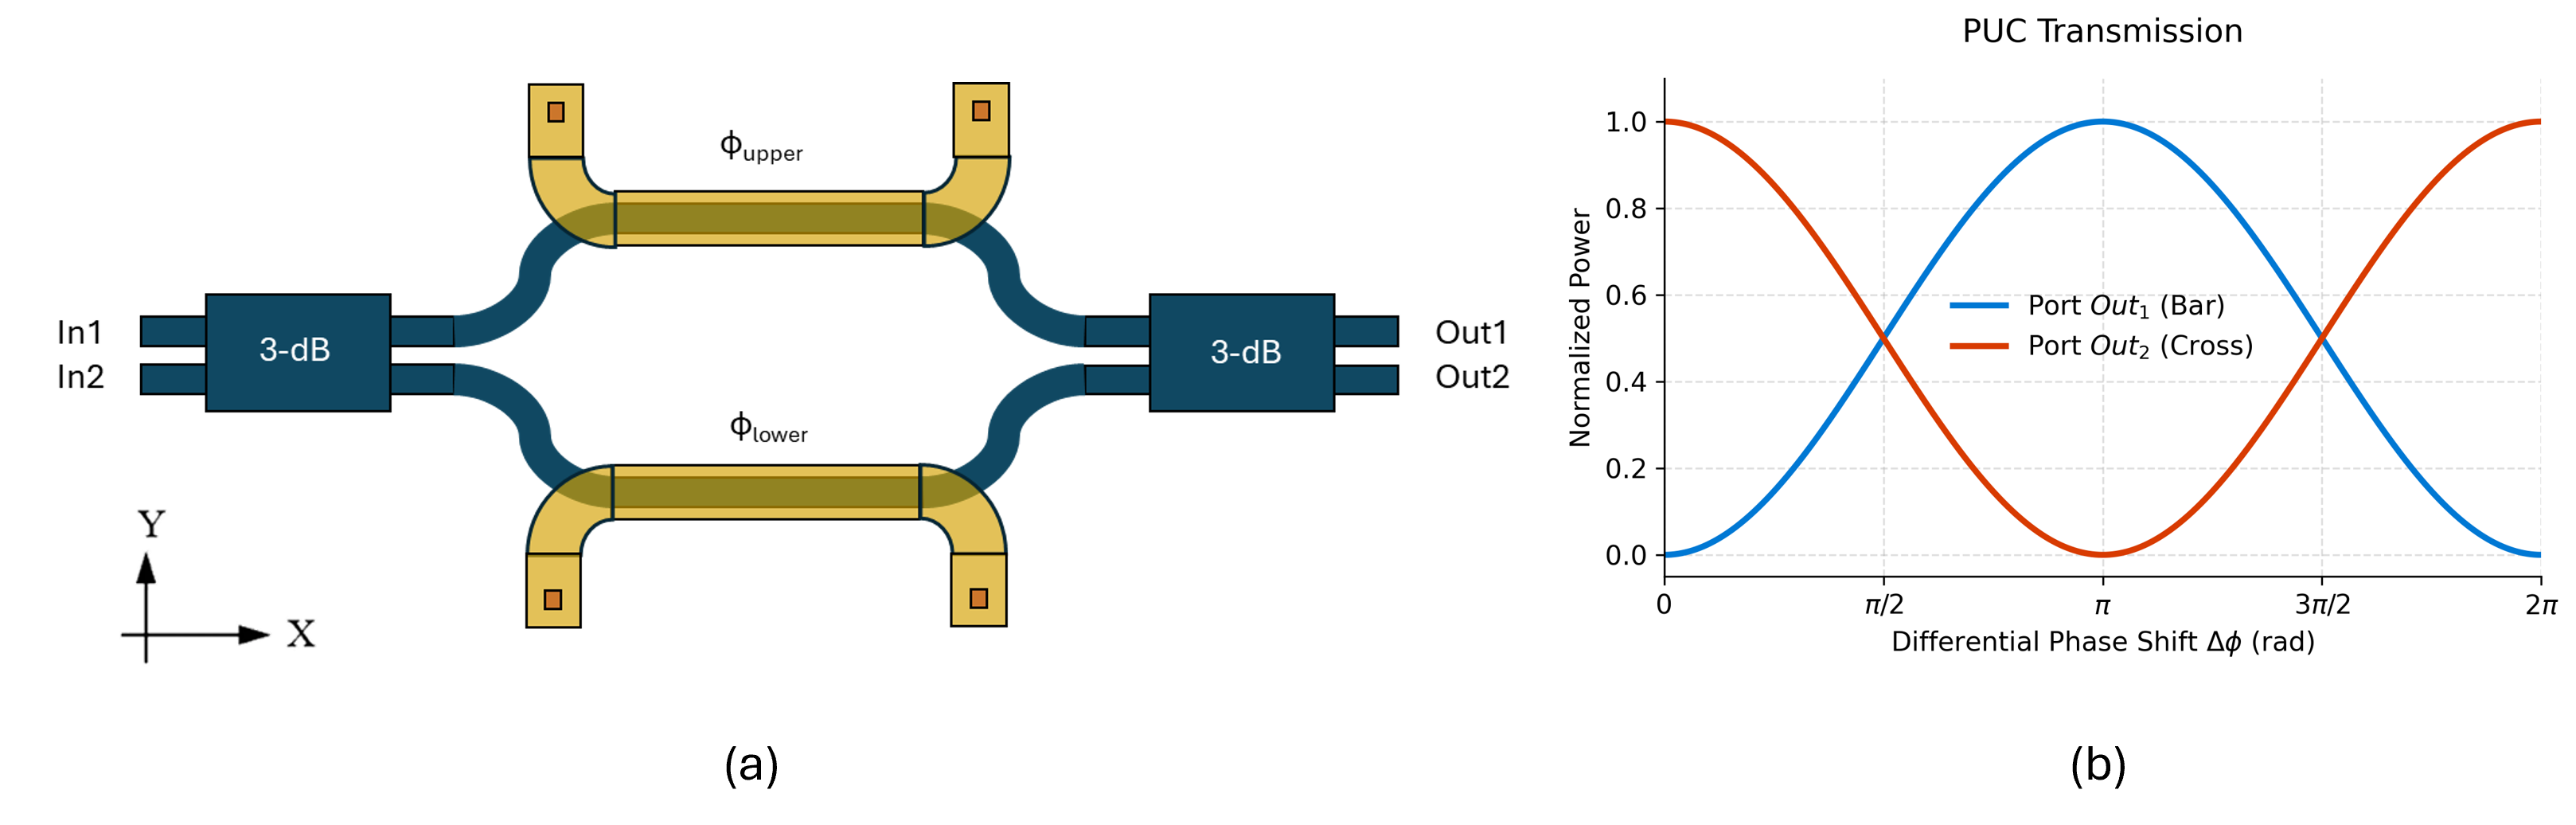
\includegraphics[width=\textwidth]{figures/ch2-puc}
    \caption{Symmetric $2 \times 2$ programmable unit cell: (a) Schematic 
    architecture showing the dual-drive MZI configuration with phase shifters $\phi_{upper}$ and 
    $\phi_{lower}$. (b) Simulated transmission characteristics showing the normalized power 
    evolution and the periodic transition between Bar and Cross states as a function of 
    $\Delta\phi$.}
    \label{fig:ch2-puc}
\end{figure}

\FloatBarrier


\section{Concluding Remarks}
\label{sec:ch2-concluding-remarks}

In this chapter, we have established the theoretical and physical foundations required to 
understand and design programmable photonic integrated circuits. Starting from the fundamental 
principles of light propagation in silicon waveguides, we analyzed the primary mechanisms for phase 
modulation, specifically the thermo-optic effect and the plasma dispersion effect in silicon
structures.

The core of the chapter focused on the Programmable Unit Cell (PUC), modeled as a symmetric 
Mach-Zehnder Interferometer. By applying the transfer matrix formalism, we derived the mathematical 
operator $\mathbf{T}_{\text{PUC}}$, which relates the input and output electric fields as a 
function of the differential phase $\Delta\phi$. This analysis confirmed that:
\begin{itemize}
    \item The unit cell naturally operates in the Cross state when no external stimulus is applied 
    ($\Delta\phi = 0$).
    \item A physical phase shift of $\pi$ radians is required to transition to the Bar state.
    \item These two degrees of freedom (amplitude via $\Delta\phi$ and common phase) allow the PUC 
    to perform the unitary transformations necessary for optical signal processing.
\end{itemize}

With the mathematical framework and the ideal behavior of the unit cell now defined, the next 
logical step is to address its physical realization. In the following chapter, we will detail the 
design, simulation, and optimization of the specific silicon photonic building blocks (MMIs, 
phase shifters, and couplers) that constitute the hardware layer of these programmable processors.

